\documentclass[10pt,compress]{beamer} % Change 10pt to make fonts of a different size
\mode<presentation>

\usepackage[spanish]{babel}
\usepackage{fontspec}
\usepackage{tikz}
\usepackage{etoolbox}
\usepackage{xcolor}
\usepackage{xstring}
\usepackage{listings}

\usetheme{UAH}
\usecolortheme{UAH}
\setbeamertemplate{navigation symbols}{} 
\setbeamertemplate{caption}[numbered]

%%%%%%%%%%%%%%%%%%%%%%%%%%%%%%%%%%%%%%%%%%%%%%%%%%%%%%%%%%%%%%%%%
%% Presentation Info
\title[Técnicas de Acceso al Medio]{Técnicas de Acceso al Medio}
\author{Enrique Alexandre}
\institute{Dpto. de Teoría de la Señal y Comunicaciones}
\date{Curso 2021/2022}
%%%%%%%%%%%%%%%%%%%%%%%%%%%%%%%%%%%%%%%%%%%%%%%%%%%%%%%%%%%%%%%%%


%%%%%%%%%%%%%%%%%%%%%%%%%%%%%%%%%%%%%%%%%%%%%%%%%%%%%%%%%%%%%%%%%
%% Descomentar para habilitar barra de navegación superior
\setNavigation
%%%%%%%%%%%%%%%%%%%%%%%%%%%%%%%%%%%%%%%%%%%%%%%%%%%%%%%%%%%%%%%%%

%%%%%%%%%%%%%%%%%%%%%%%%%%%%%%%%%%%%%%%%%%%%%%%%%%%%%%%%%%%%%%%%%
%% Configuración de logotipos en portada
%% Opacidad de los logotipos
\newcommand{\opacidad}{1}
%%%%%%%%%%%%%%%%%%%%%%%%%%%%%%%%%%%%%%%%%%%%%%%%%%%%%%%%%%%%%%%%%

%%%%%%%%%%%%%%%%%%%%%%%%%%%%%%%%%%%%%%%%%%%%%%%%%%%%%%%%%%%%%%%%%
%% FOOTLINE
%% Comment/Uncomment the following blocks to modify the footline
%% content in the body slides. 
%% Option A: Title and institute
\footlineA
%%%%%%%%%%%%%%%%%%%%%%%%%%%%%%%%%%%%%%%%%%%%%%%%%%%%%%%%%%%%%%%%%

\begin{document}

%%%%%%%%%%%%%%%%%%%%%%%%%%%%%%%%%%%%%%%%%%%%%%%%%%%%%%%%%%%%%%%%%
% Use this block for a blue title slide with modified footline
{\titlepageBlue
    \begin{frame}
        \titlepage
    \end{frame}
}

{
\disableNavigation{white}
\begin{frame}[shrink]{Índice}
 \frametitle{Índice}
 \tableofcontents
  % You might wish to add the option [pausesections]
\end{frame}
}

\section{Introducción}

\subsection{Motivación}

\begin{frame}{Introducción}{Motivación}
    \begin{itemize}
		\item Recursos escasos en un sistema de telecomunicación
		\begin{itemize}
			\item Ancho de banda
      \item Potencia
      \item Número de portadoras disponibles
		\end{itemize}
    \item ¿Qué se hace cuando varios usuarios quieren acceder a estos recursos?
    \begin{itemize}
			\item Dividir y asignar dichos recursos
      \begin{itemize}
        \item Frecuencia
        \item Tiempo
        \item Código
      \end{itemize}
		\end{itemize}
	\end{itemize}
\end{frame}

\subsection{Distintas aproximaciones}
\begin{frame}{Introducción}{Distintas aproximaciones}
  \begin{columns}[onlytextwidth]
    \begin{column}{.5\textwidth}
      \begin{itemize}
        \item {\bf MAC} (Multiple-Access Channel)
        \begin{itemize}
          \item Ej.: GSM, Wi-Fi
        \end{itemize}
        \vspace{1cm}
        \item {\bf BC} (Broadcast Channel)
        \begin{itemize}
          \item Ej.: Radio, TV
        \end{itemize}
        \vspace{1cm}
        \item {\bf IC} (Interference Channel)
        \begin{itemize}
          \item Ej.: Redes militares
        \end{itemize}
      \end{itemize}
    \end{column}
    \begin{column}{.5\textwidth}
      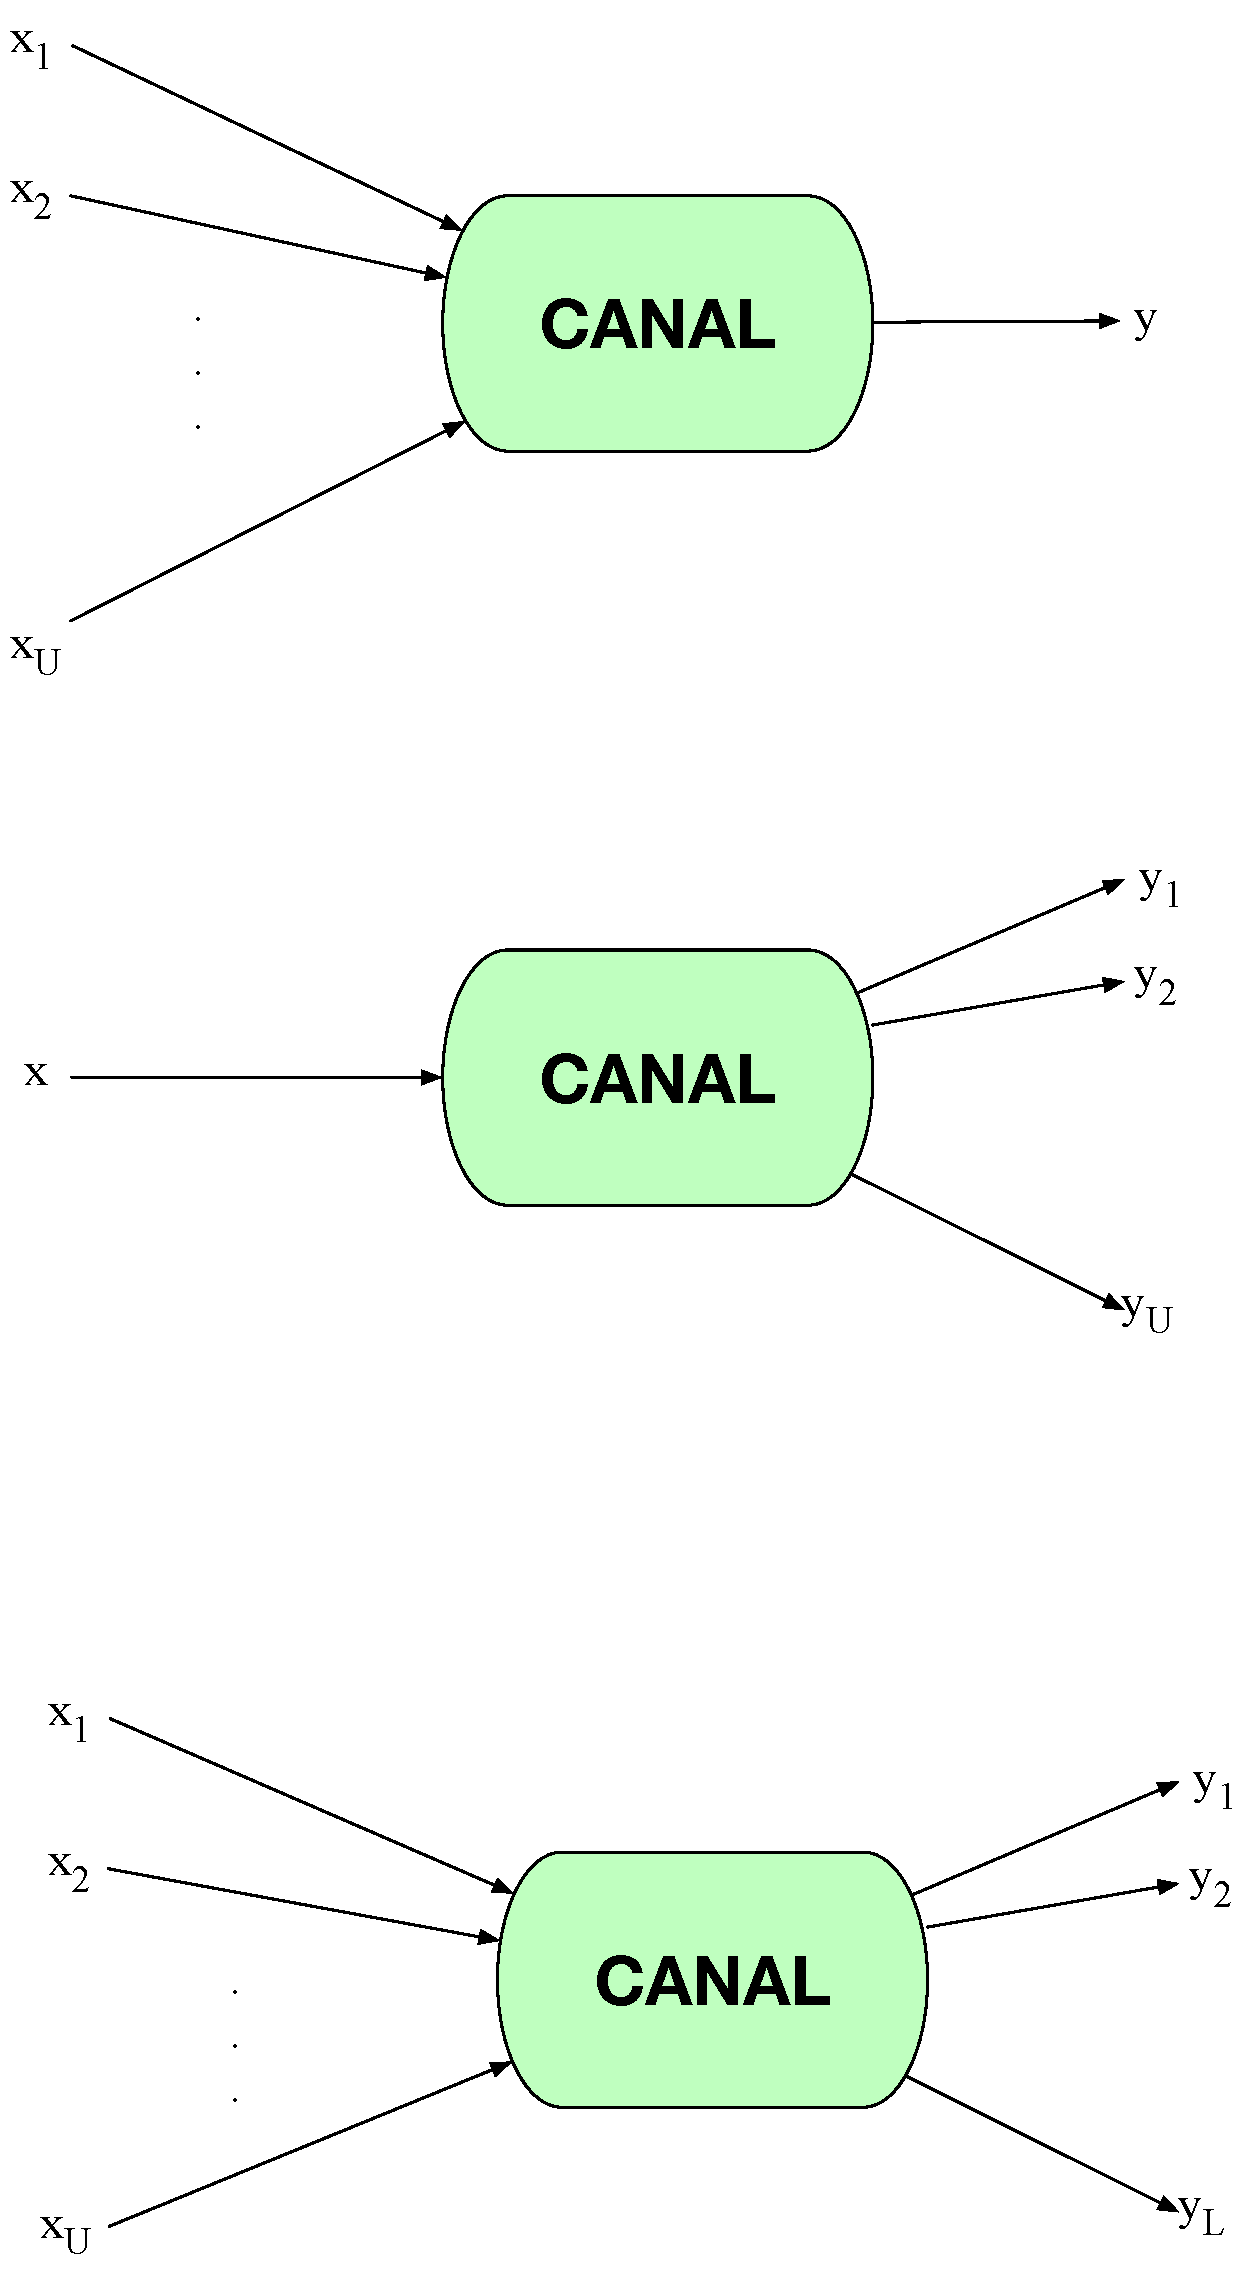
\includegraphics[width=0.6\linewidth]{../Apuntes/Figuras/ModosDeAcceso.pdf}
    \end{column}
  \end{columns}
\end{frame}



\subsection{Representación intuitiva}
\begin{frame}{Introducción}{Representación intuitiva}
  \begin{tabular}{ccc}
    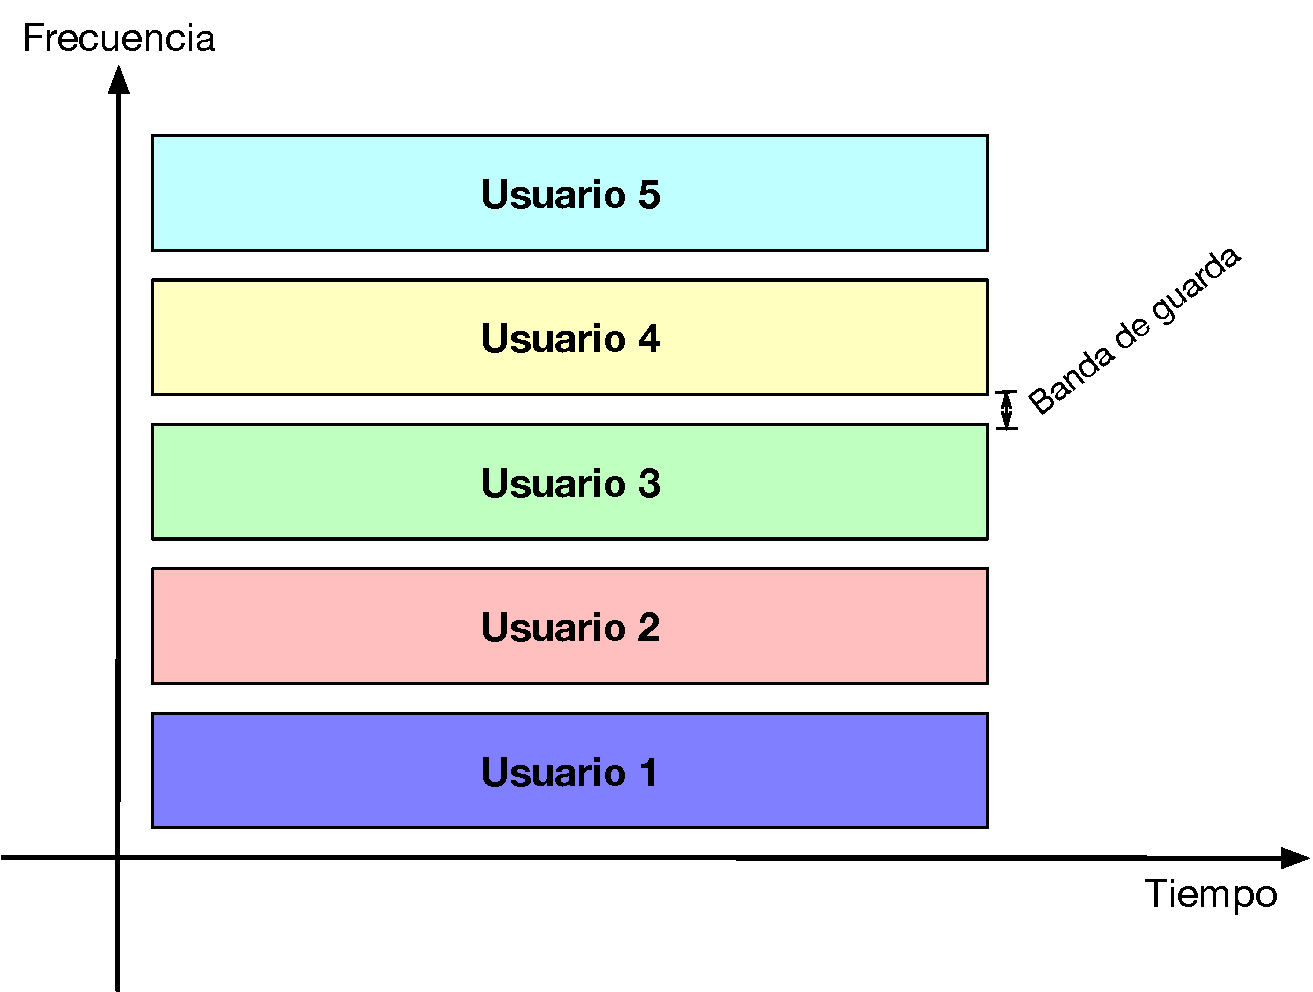
\includegraphics[width=0.3\linewidth]{../Apuntes/Figuras/FDMA.pdf} & 
    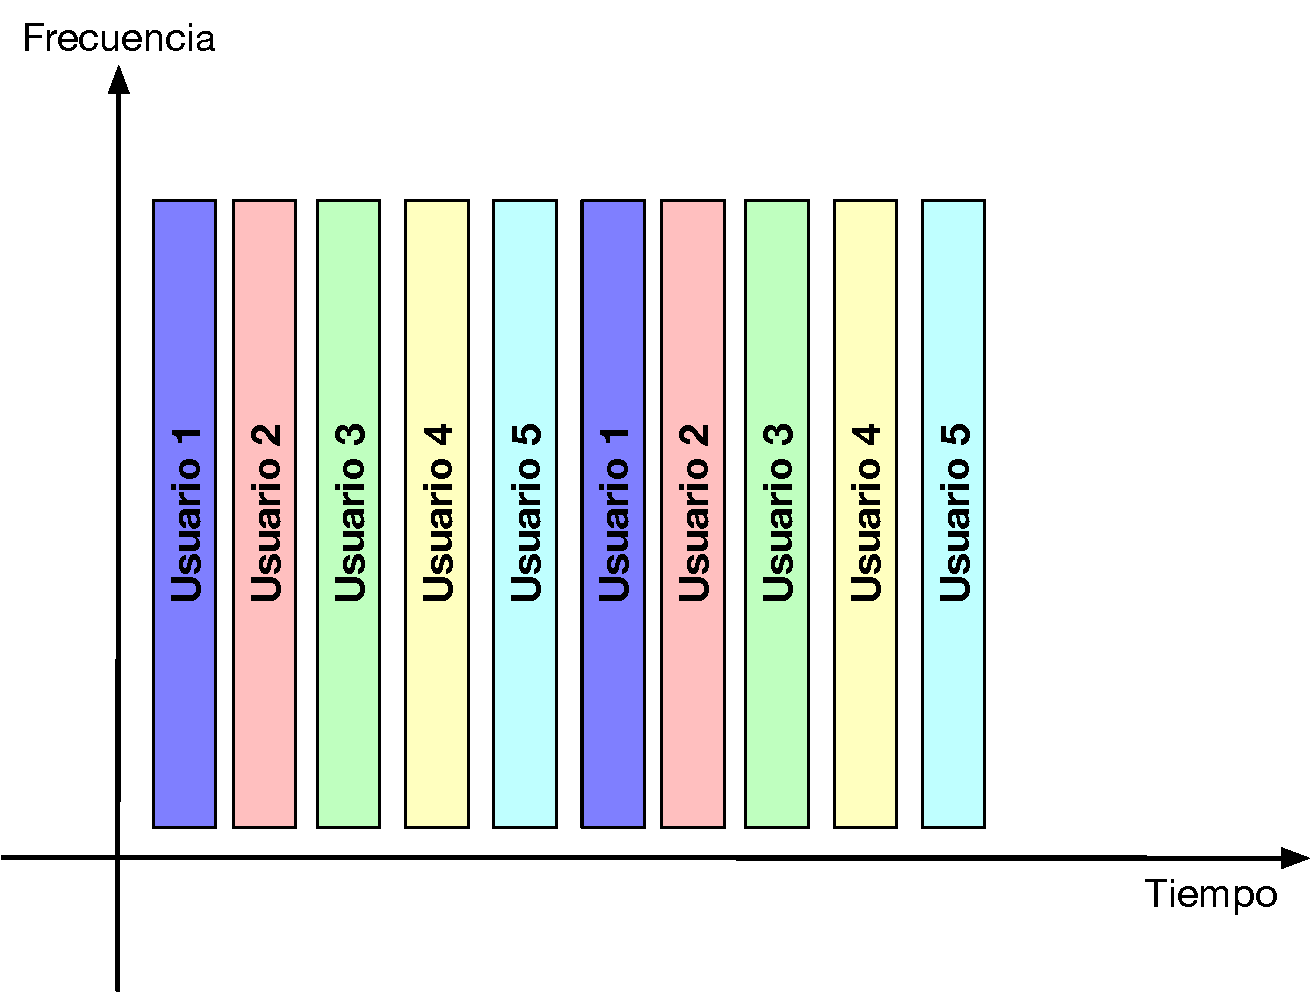
\includegraphics[width=0.3\linewidth]{../Apuntes/Figuras/TDMA.pdf} & 
    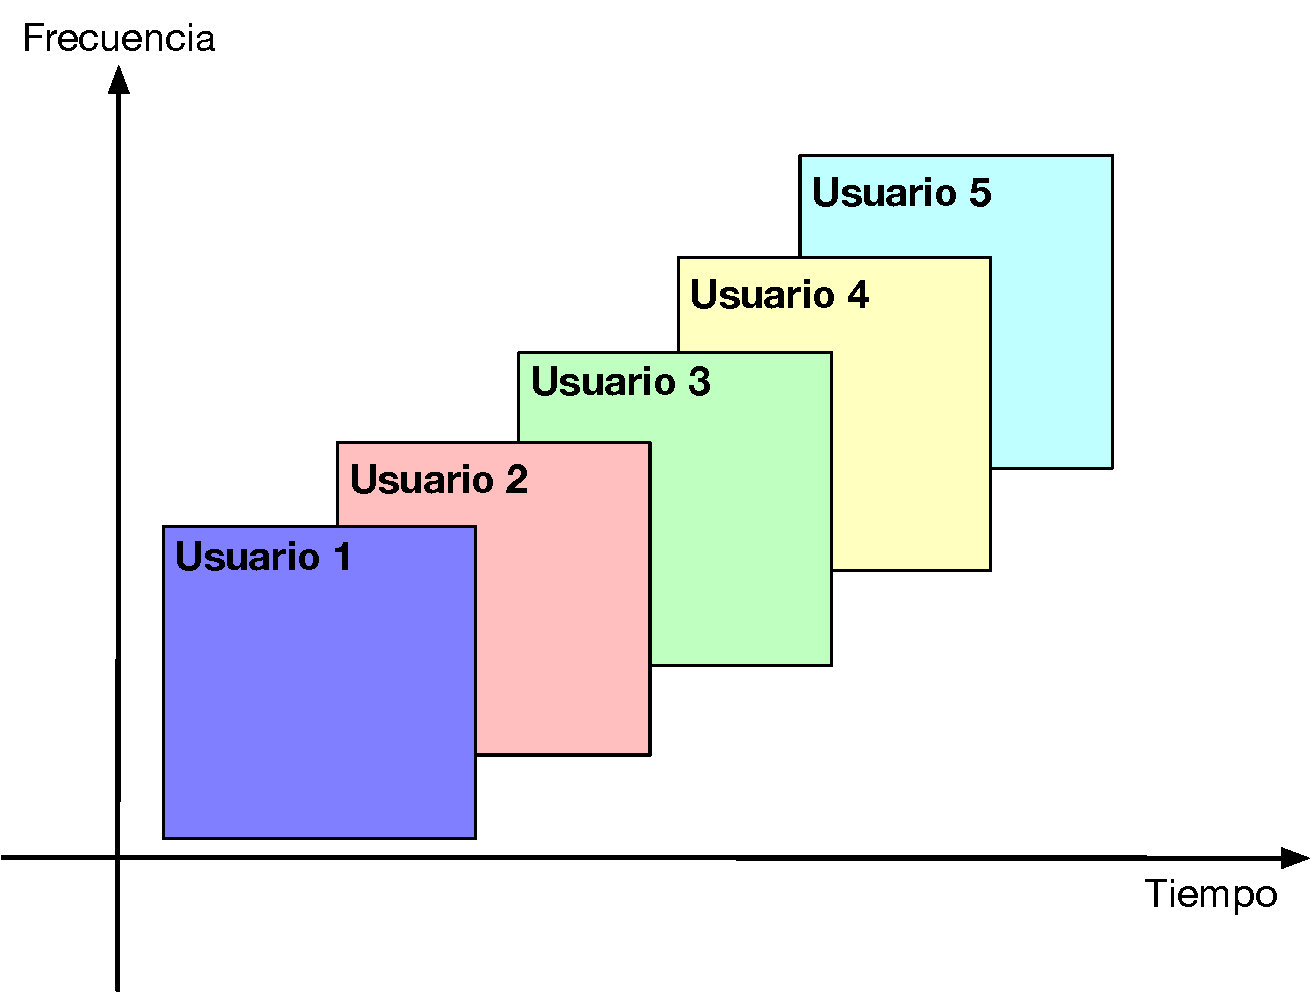
\includegraphics[width=0.3\linewidth]{../Apuntes/Figuras/CDMA.pdf} \\
    {\bf FDMA} & {\bf TDMA} & {\bf CDMA} \\
    A cada usuario se le   & A cada usuario se le & A cada usuario se le \\
    asigna una frecuencia & asigna un slot de tiempo & asigna un código\\
  \end{tabular}

\end{frame}

\subsection{Ejemplo: telefonía móvil}
\begin{frame}{Introducción}{Ejemplo: telefonía móvil}
  \begin{itemize}
    \item {\bf 1G}: FDMA
    \item {\bf 2.xG}: TDMA (con alguna variación)
    \item {\bf 3.xG}: CDMA
    \item {\bf 4G}: OFDMA + MIMO
    \item {\bf 5G}: NOMA
  \end{itemize}
\end{frame}

\section{FDMA}

\subsection{Introducción}
\begin{frame}{FDMA (Frequency Division Multiple Access)}{Definición}
	\centering 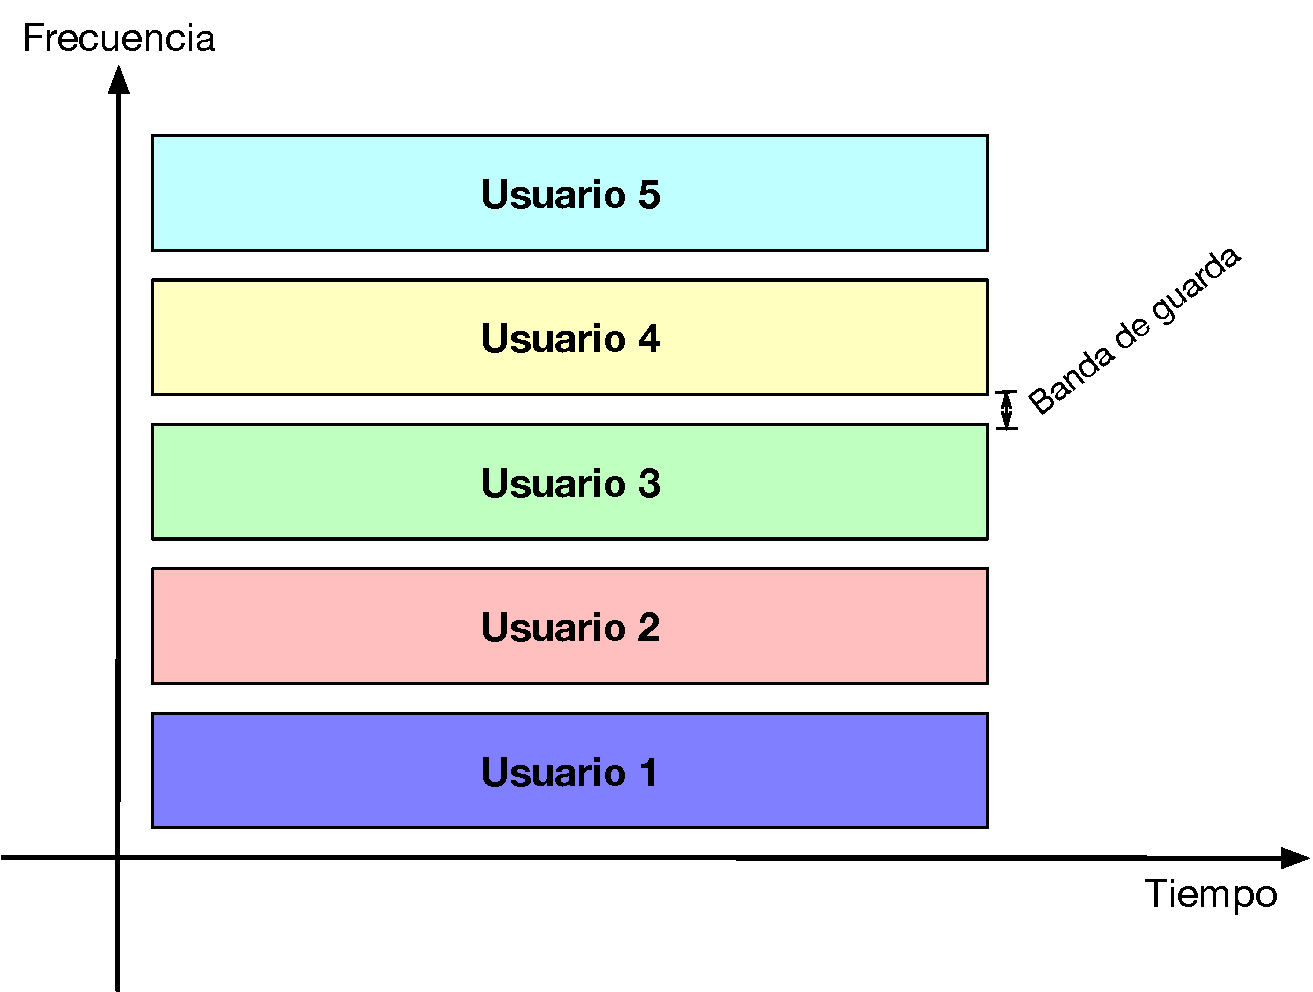
\includegraphics[width=0.8\linewidth]{../Apuntes/Figuras/FDMA.pdf}
\end{frame}

\subsection{Modo full duplex}
\begin{frame}{FDMA}{Modo full duplex}
  \centering 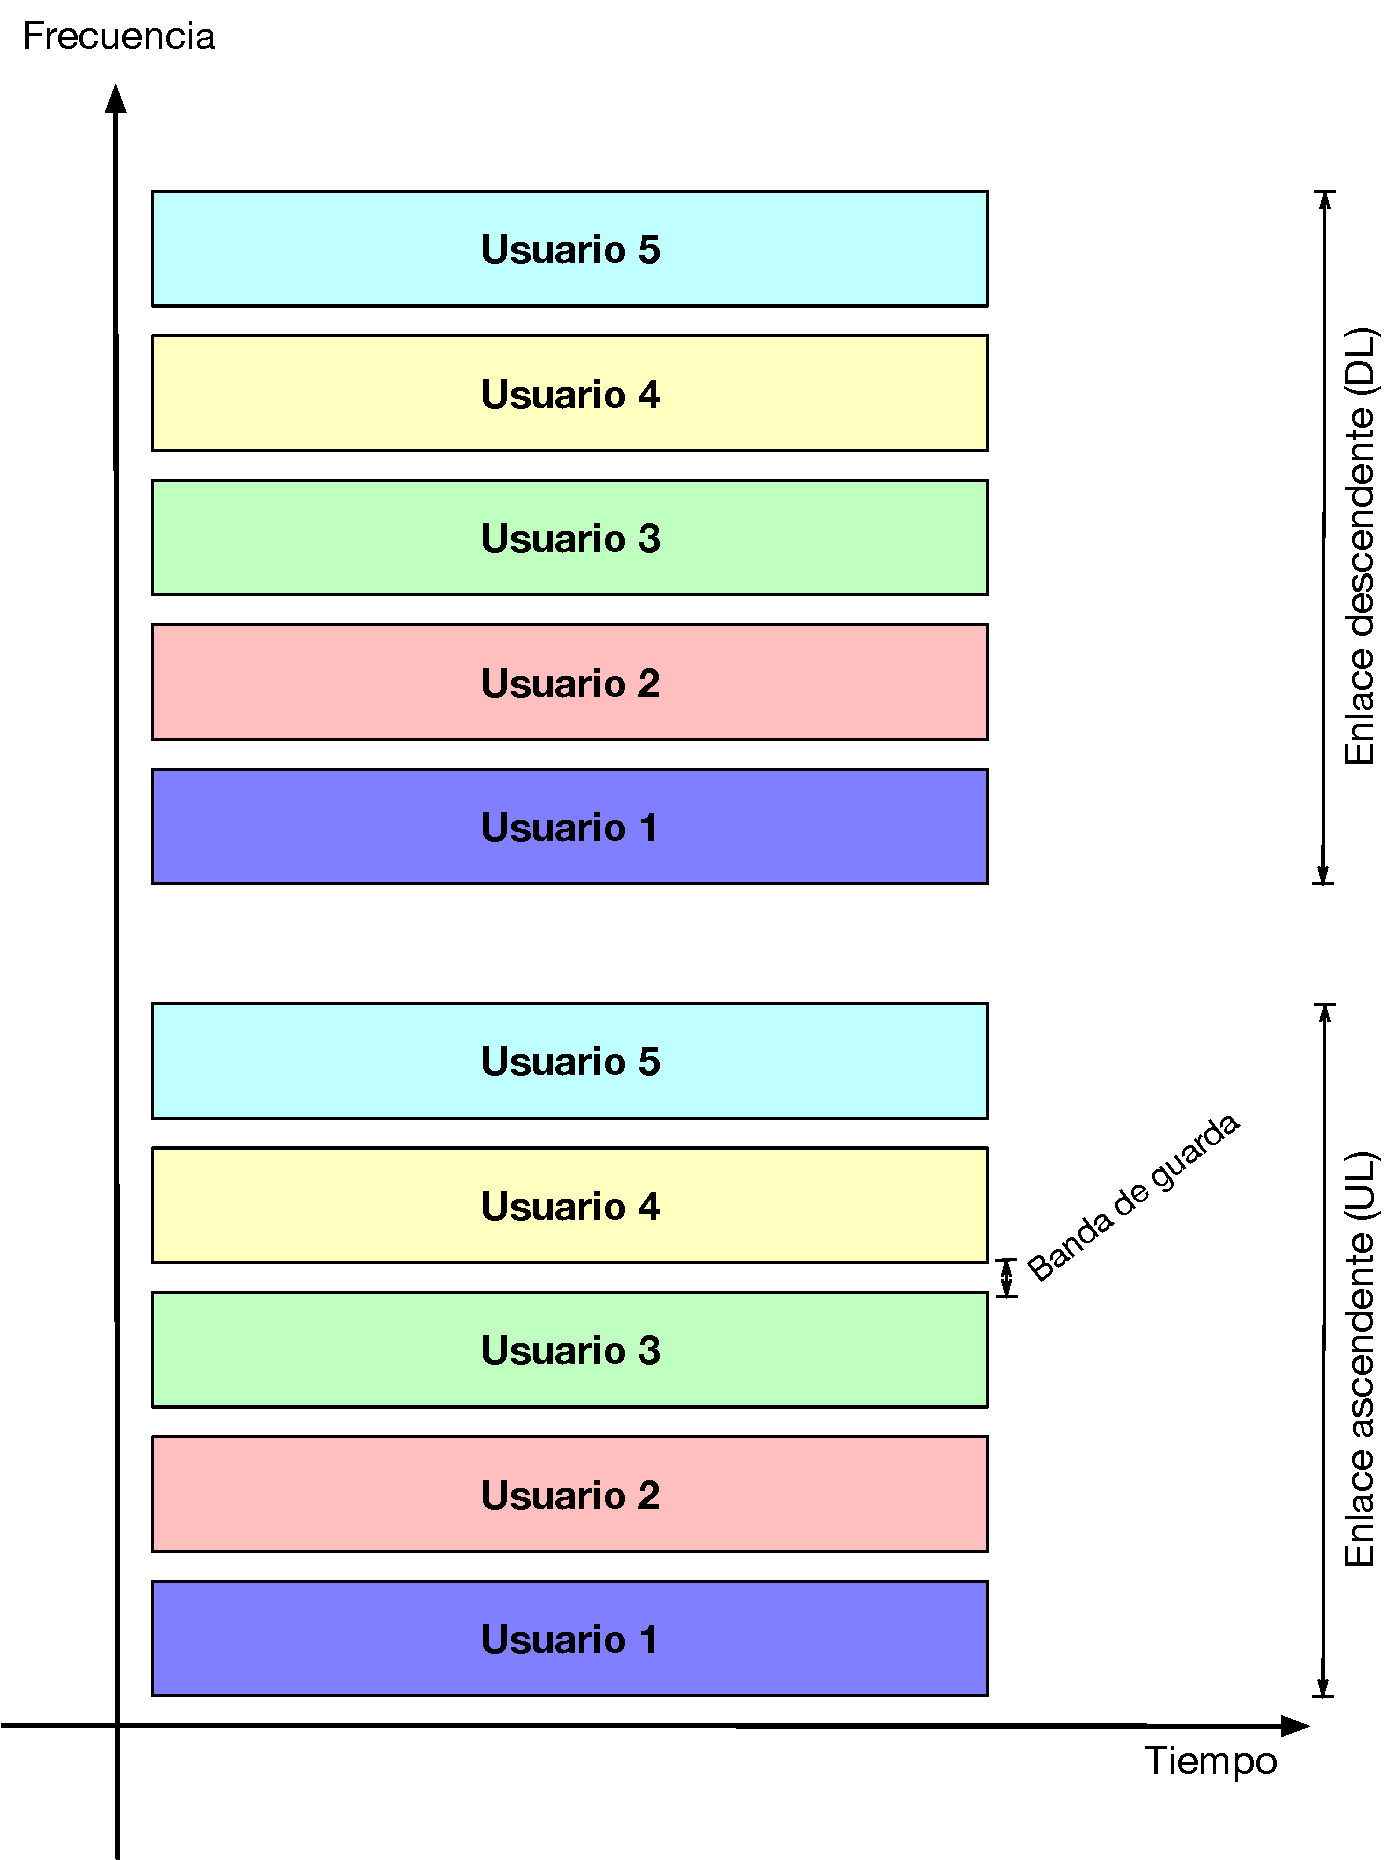
\includegraphics[width=0.4\linewidth]{../Apuntes/Figuras/FDMA_FD.pdf}
\end{frame}

\subsection{Ventajas e inconvenientes}
\begin{frame}{FDMA}{Ventajas e inconvenientes}
  \begin{itemize}
    \item Ventajas:
      \begin{itemize}
        \item Compatible con modulaciones analógicas y digitales
        \item Implementación muy sencilla
      \end{itemize}
    \item Inconvenientes:
      \begin{itemize}
        \item No aprovecha bien el espectro disponible (en comparación con TDMA y CDMA)
        \item Es un sistema rígido
        \item Posible interferencia entre canales
      \end{itemize}
    \item Aplicaciones:
      \begin{itemize}
        \item FM comercial: BW=150kHz, guarda de 25kHz
        \item Fibra óptica
      \end{itemize}
  \end{itemize}
\end{frame}


\section{TDMA}
\subsection{Introducción}
\begin{frame}{TDMA (Time Division Multiple Access)}{Introducción}
  \centering 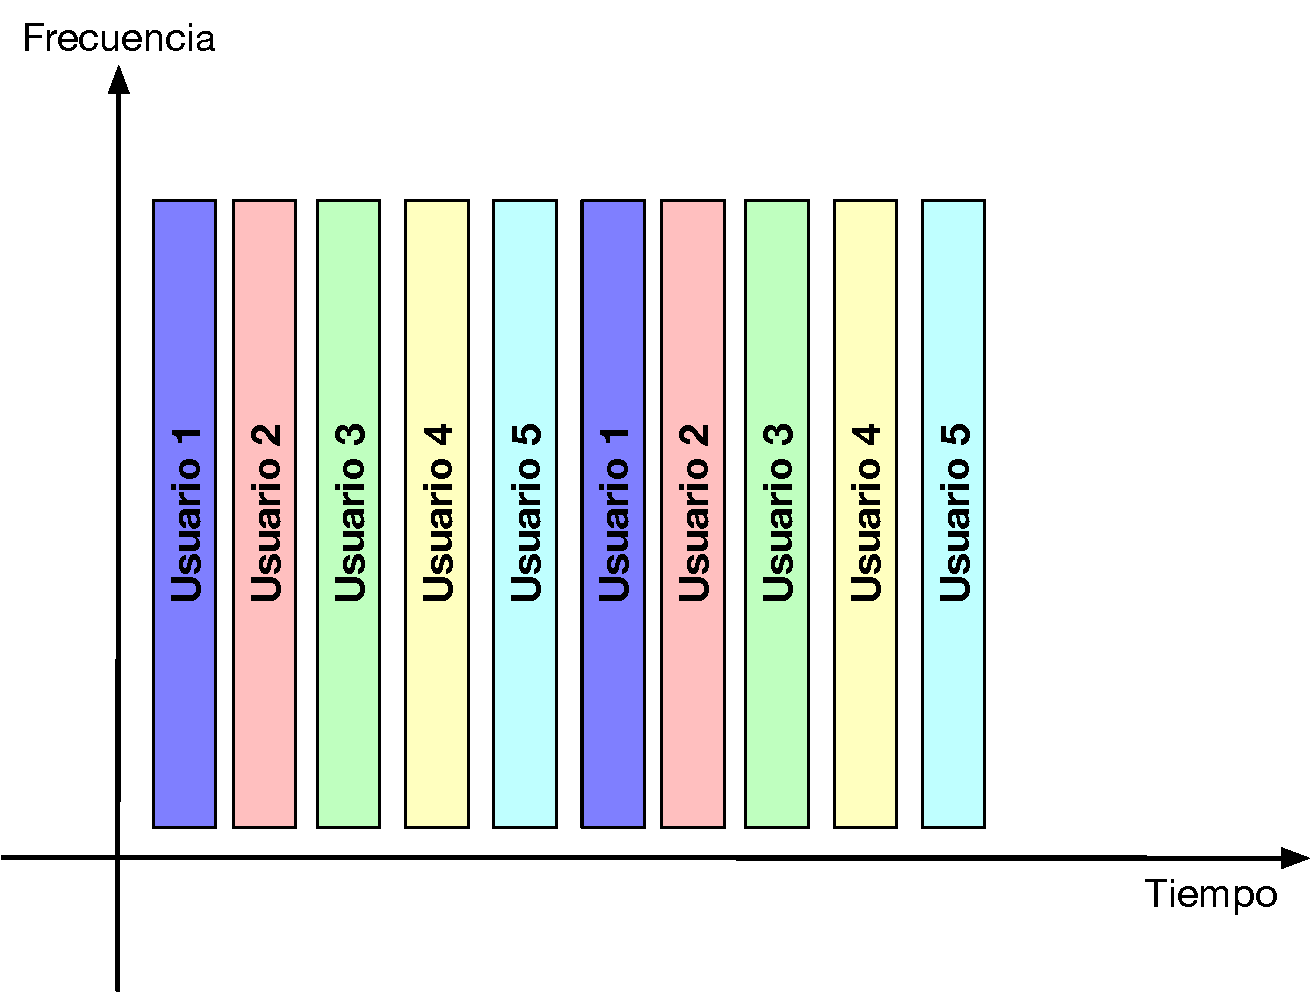
\includegraphics[width=0.8\linewidth]{../Apuntes/Figuras/TDMA.pdf}
\end{frame}

\subsection{Parámetros importantes} 
\begin{frame}{TDMA}{Parámetros importantes}
  \centering 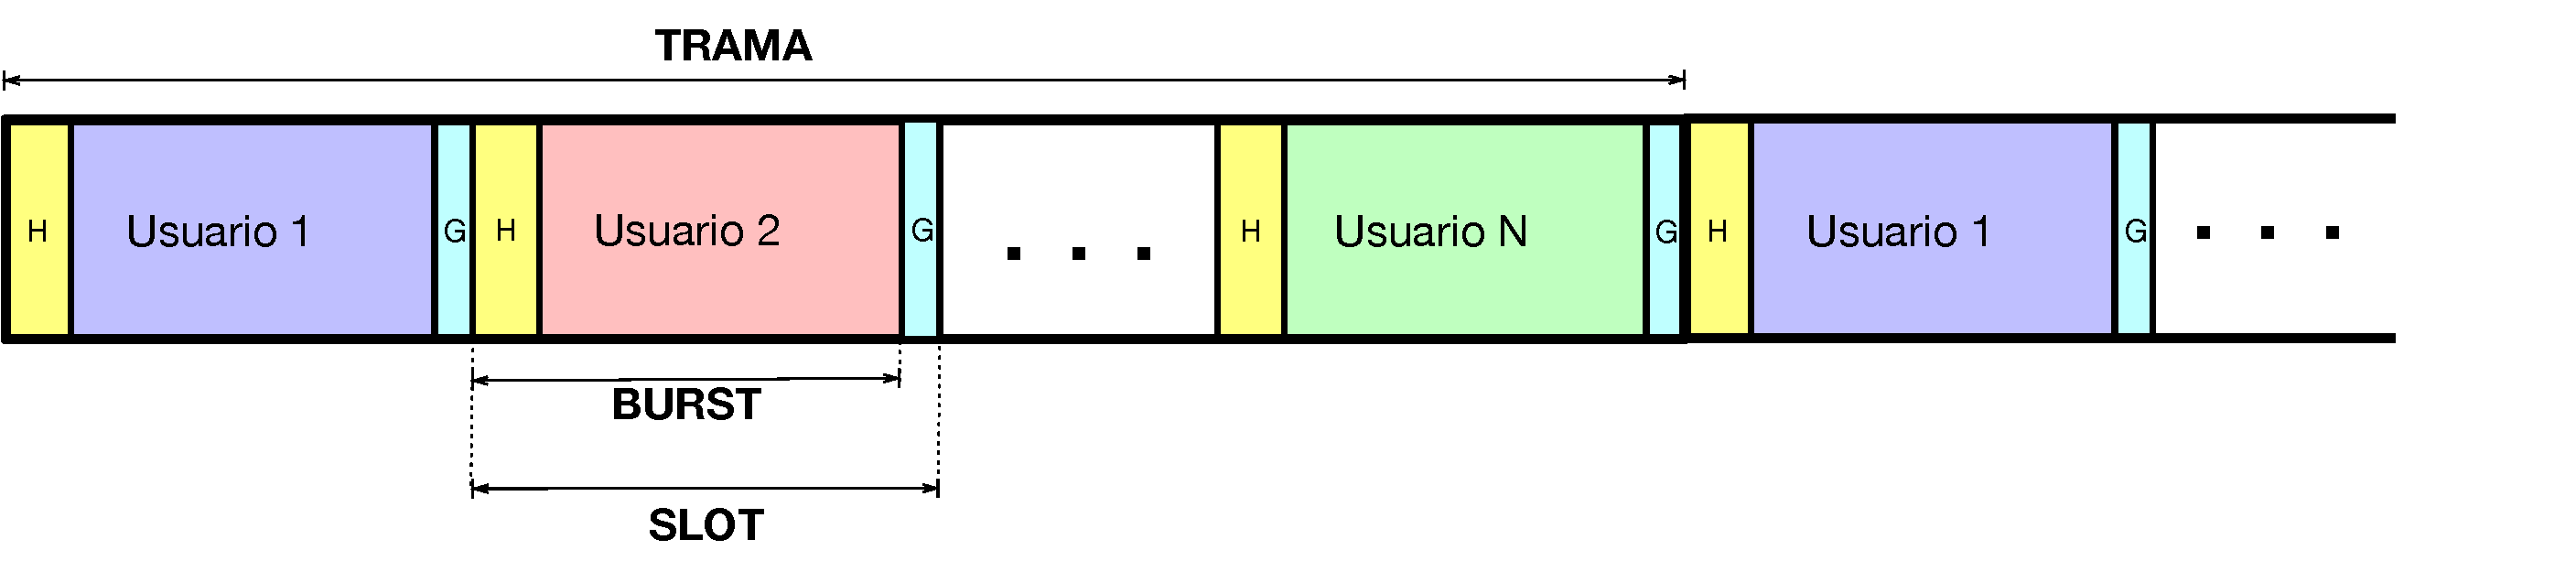
\includegraphics[width=0.8\linewidth]{../Apuntes/Figuras/TramasTDMA.pdf}
  \begin{itemize}
    \item $B_{TRAMA}$, $T_{TRAMA}$: Nº de bits y duración de la trama
    \item $N$: Nº de slots por trama
    \item $B_{SLOT}$: Nº de bits en cada slot
    \item $B_{BURST}$: Nº de bits de información por burst:\\
      $B_{BURST} = B_{SLOT} - G$
    \item $H$: Bits de overhead por slot
    \item $G$: Bits/tiempo de guarda
  \end{itemize}
\end{frame}

\subsection{Ejemplo: GSM}
\begin{frame}{TDMA}{Ejemplo: GSM}
  \centering 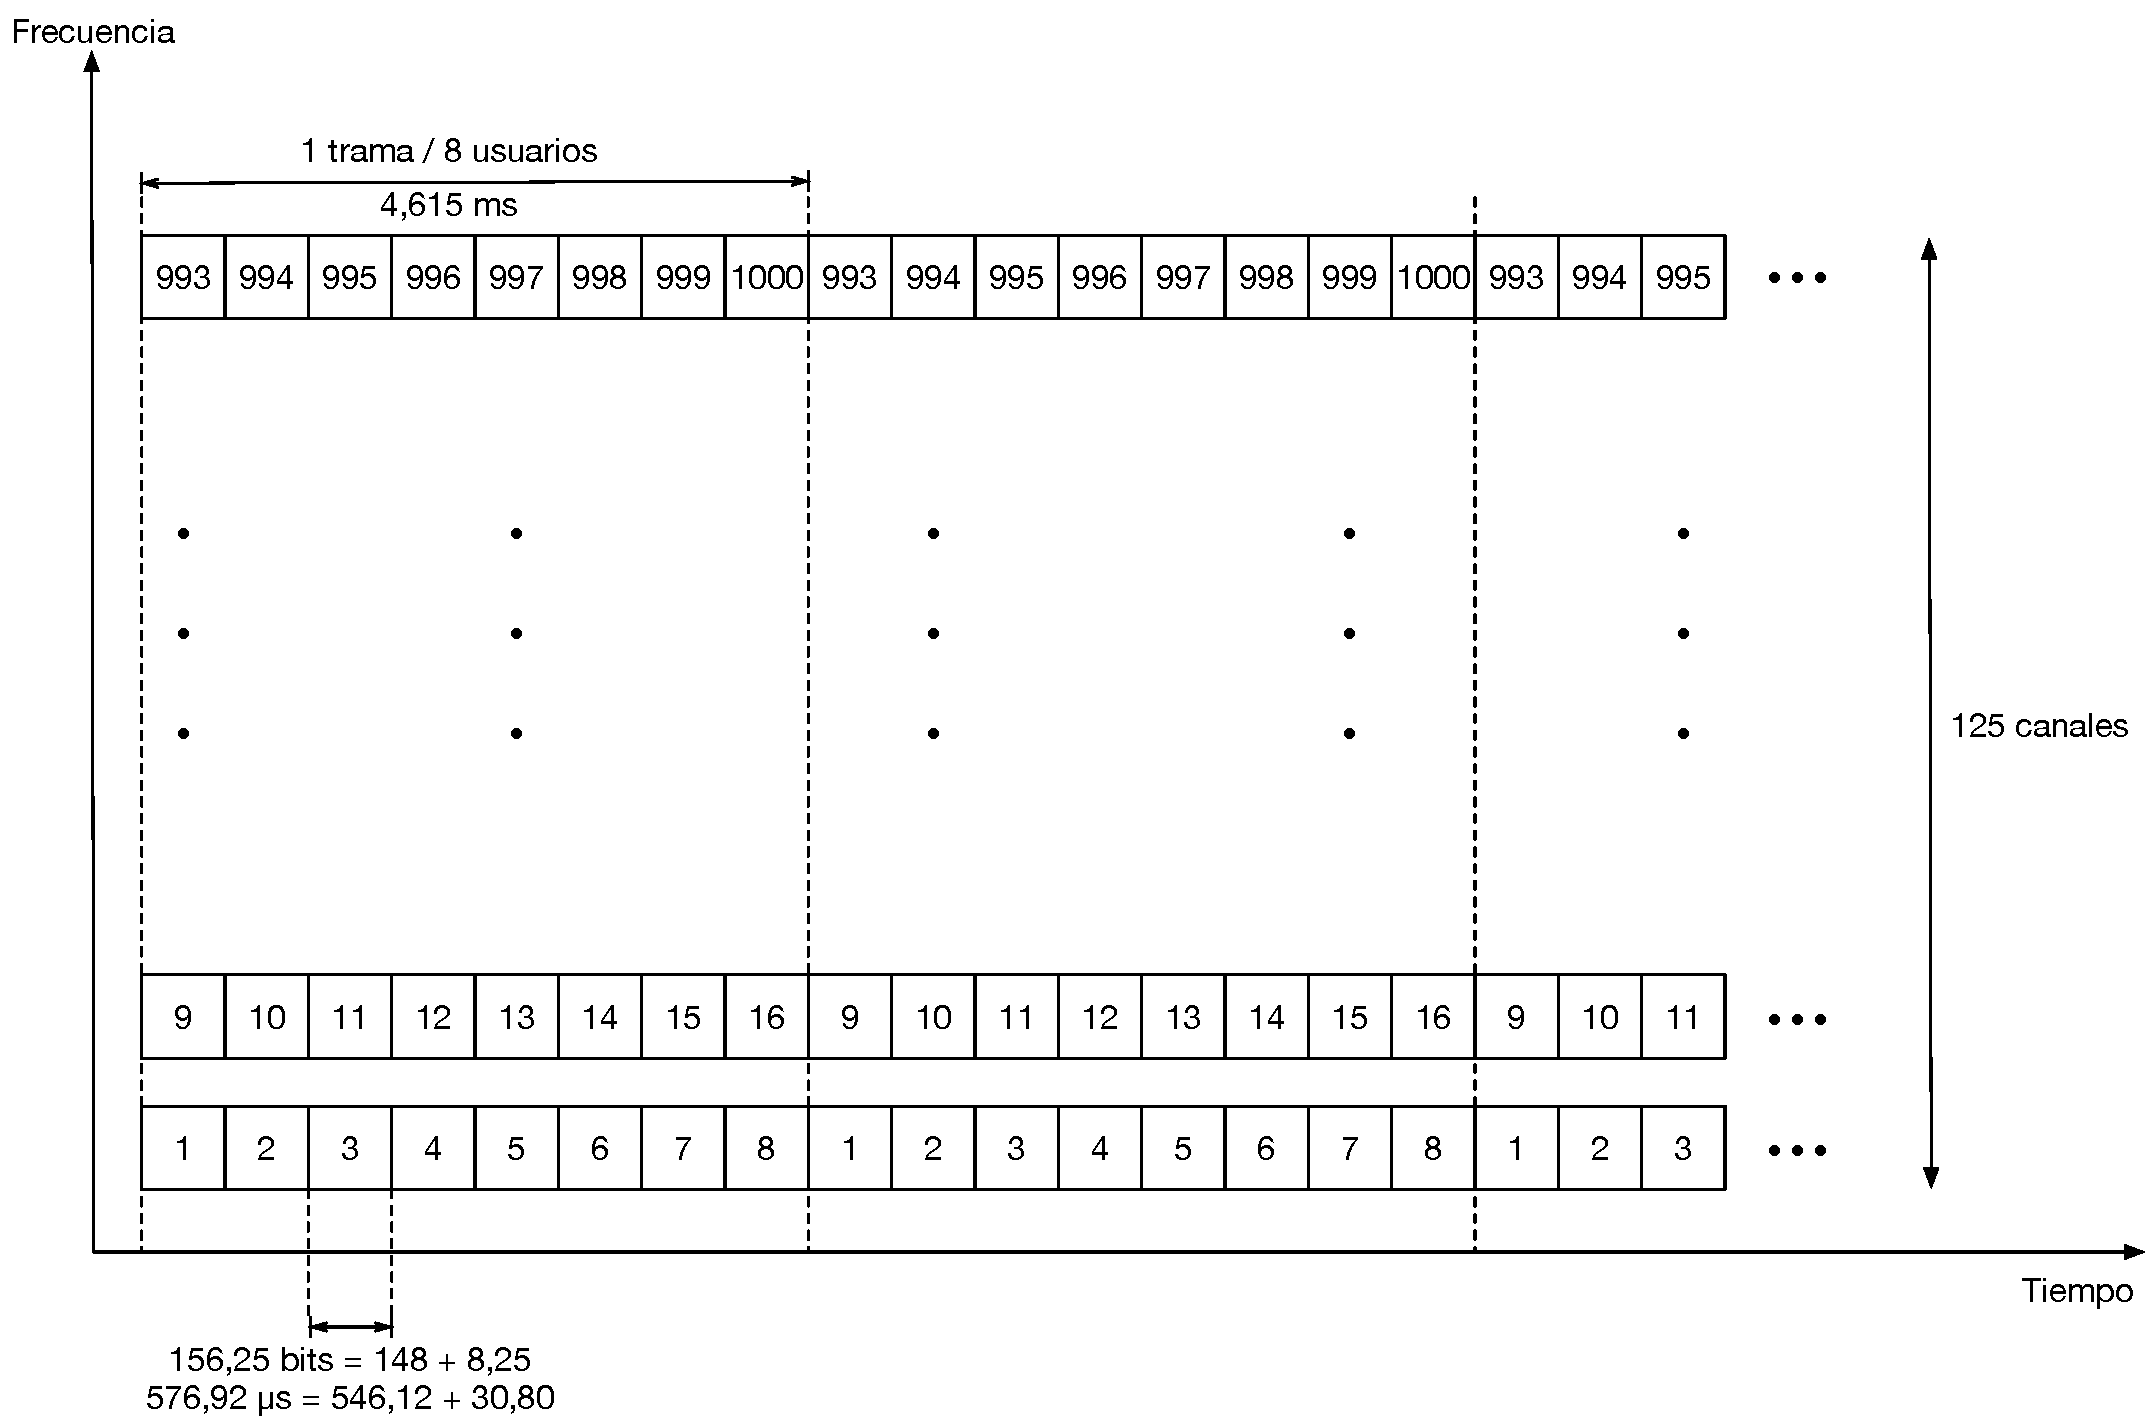
\includegraphics[width=0.8\linewidth]{../Apuntes/Figuras/AccesoAlMedioGSM.pdf}
\end{frame}

\subsection{Ejemplo: GSM}
\begin{frame}{TDMA}{Ejemplo: GSM}
  \centering 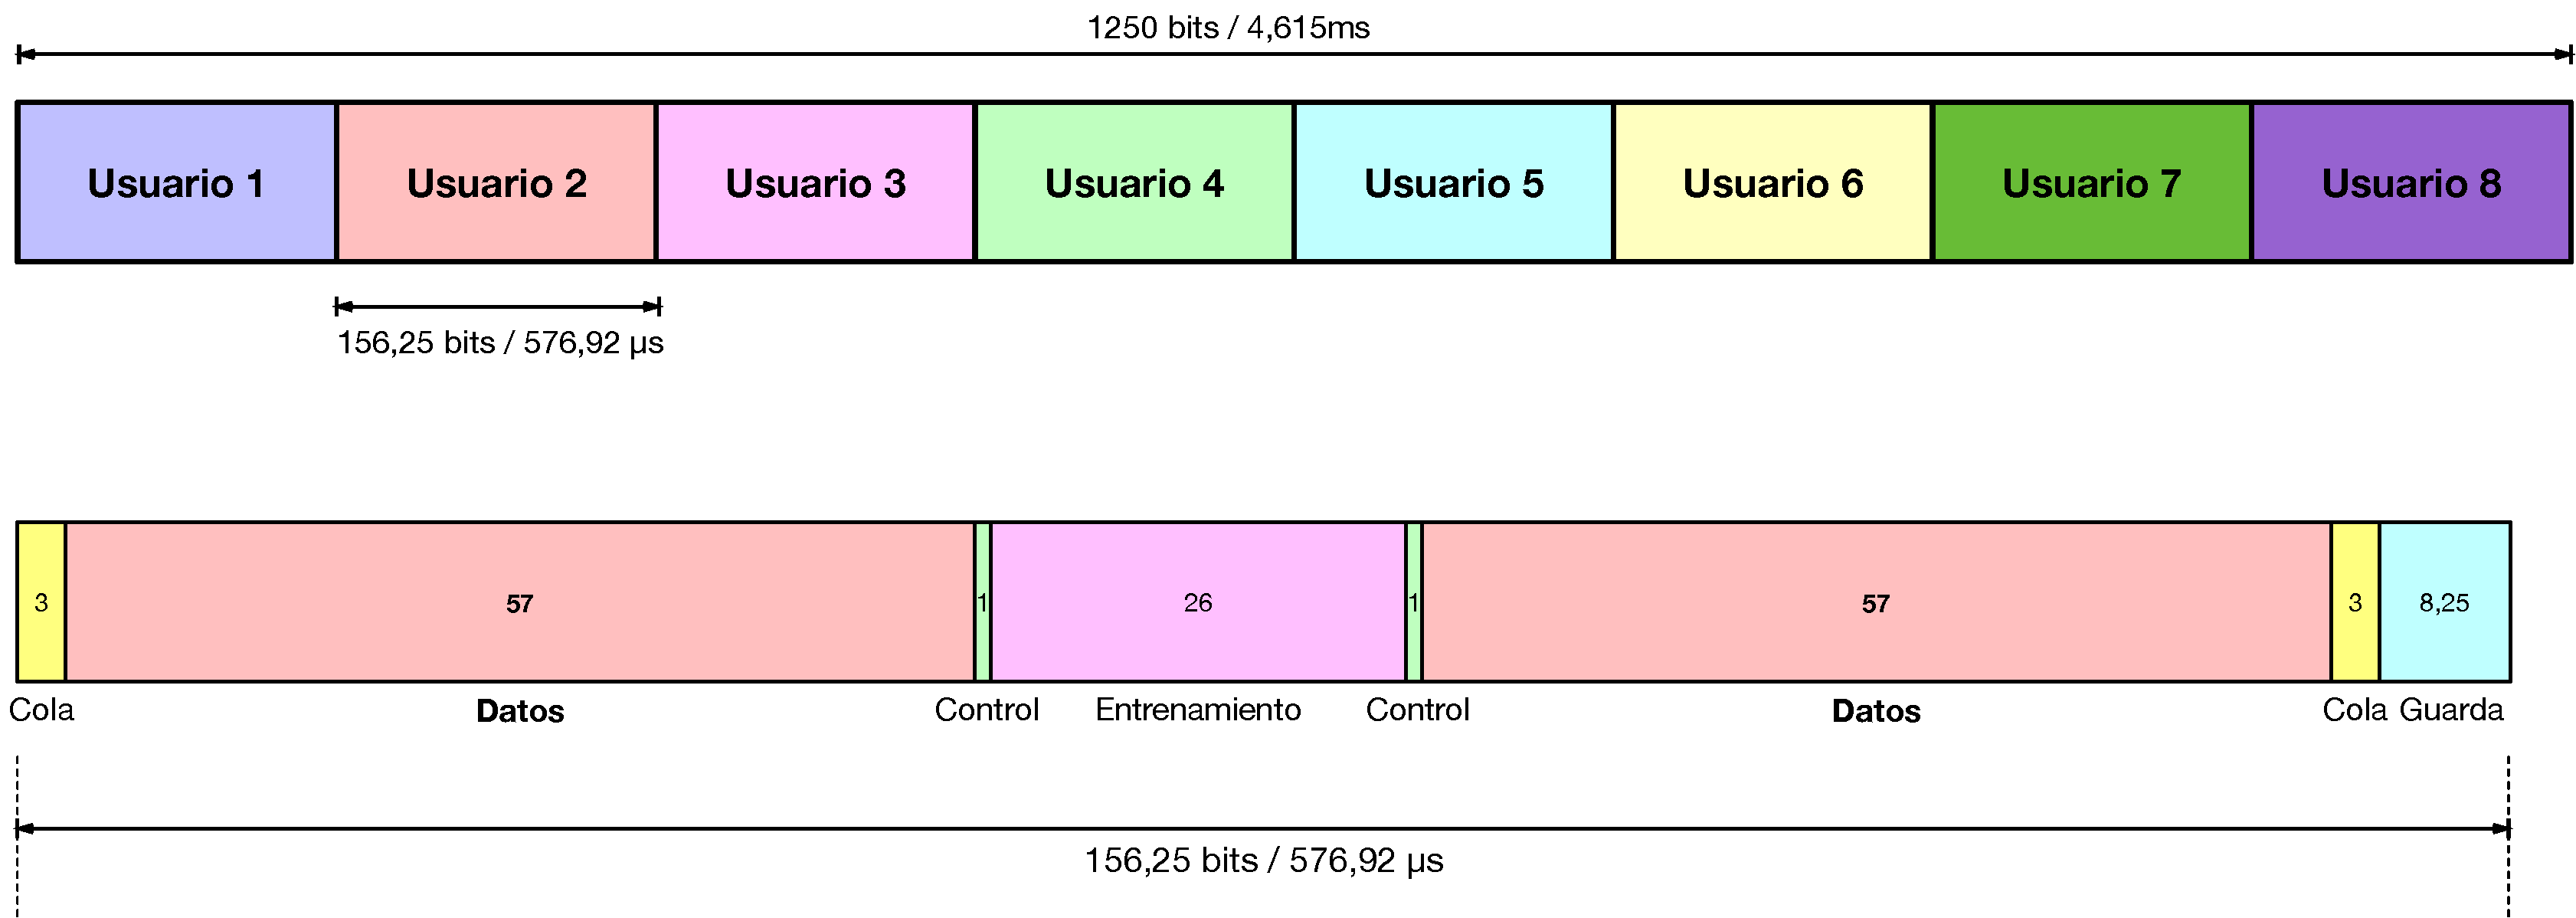
\includegraphics[width=0.7\linewidth]{../Apuntes/Figuras/TramaGSM2.pdf}
  \begin{columns}[onlytextwidth]
    \begin{column}{.4\textwidth}
  \begin{itemize}
    \item $B_{SLOT} = 156,25$ bits
    \item $B_{BURST} = 148$ bits
    \item $H = 34$ bits
    \item $G = 8,25$ bits
    \item $T_{SLOT} = 576,92 \mu s$
    \item $T_{BURST} = 546,12 \mu s$
    \item $T_{TRAMA} = 4,615 ms$
  \end{itemize}
\end{column}
  \begin{column}{.6\textwidth}
    \begin{itemize}
      \item $C = \frac{B_{BURST}}{T_{BURST}} = \frac{148}{546,12} = 271 kbps$
      \item $R_{b_U} = \frac{B_{BURST}-H}{T_{TRAMA}} = \frac{114}{4,615 ms} = 24,7 kbps$
    \end{itemize}
  \end{column}
\end{columns}
\end{frame}


\subsection{Ejemplo: Enlace ascendente PON}
\begin{frame}{TDMA}{Ejemplo: Enlace ascendente PON}
  \centering 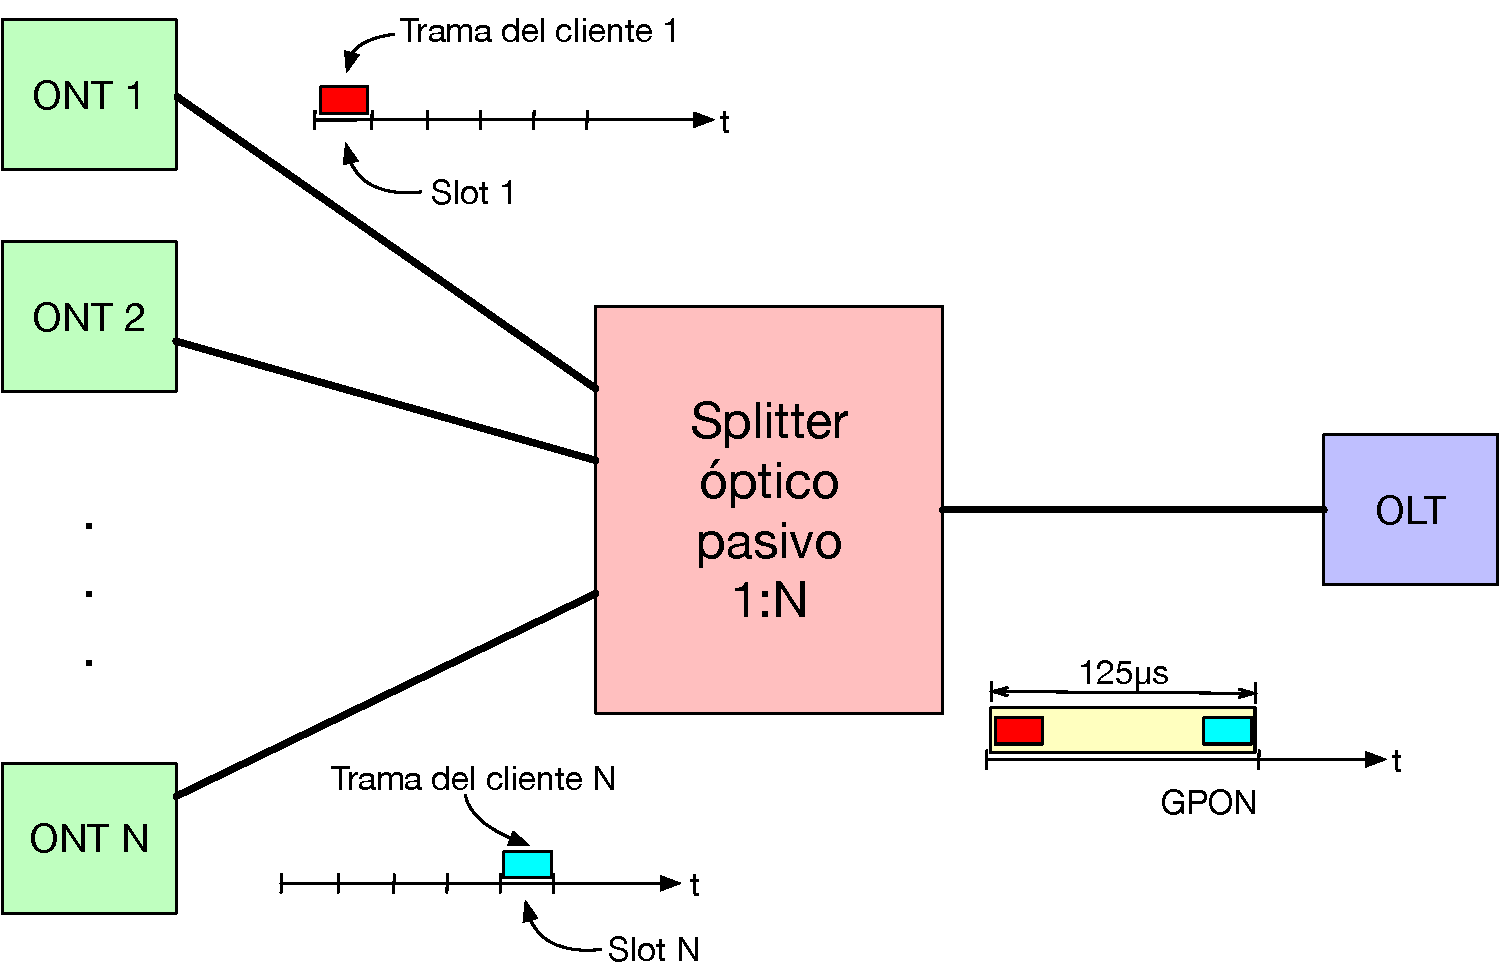
\includegraphics[width=0.8\linewidth]{../Apuntes/Figuras/TDMA_PON.pdf}
\end{frame}

\subsection{Ventajas e inconvenientes}
\begin{frame}{TDMA}{Ventajas e inconvenientes}
  \begin{itemize}
    \item Ventajas:
      \begin{itemize}
        \item Versatilidad. Se pueden asignar más o menos slots a cada usuario. 
        \item Buen rendimiento espectral
      \end{itemize}
    \item Inconvenientes:
      \begin{itemize}
        \item Complejidad. Requiere sincronización estricta
        \item Limitado a sistemas digitales
      \end{itemize}
    \item Aplicaciones:
      \begin{itemize}
        \item Telefonía móvil 2.xG (en combinación con FDMA)
      \end{itemize}
  \end{itemize}
\end{frame}


\section{SDMA}
\begin{frame}{SDMA (Spatial Division Multiple Access)}
  \begin{itemize}
    \item Se utilizan antenas directivas para cubrir distintas zonas del espacio con distintos haces de radiación.
  \end{itemize}
  \centering 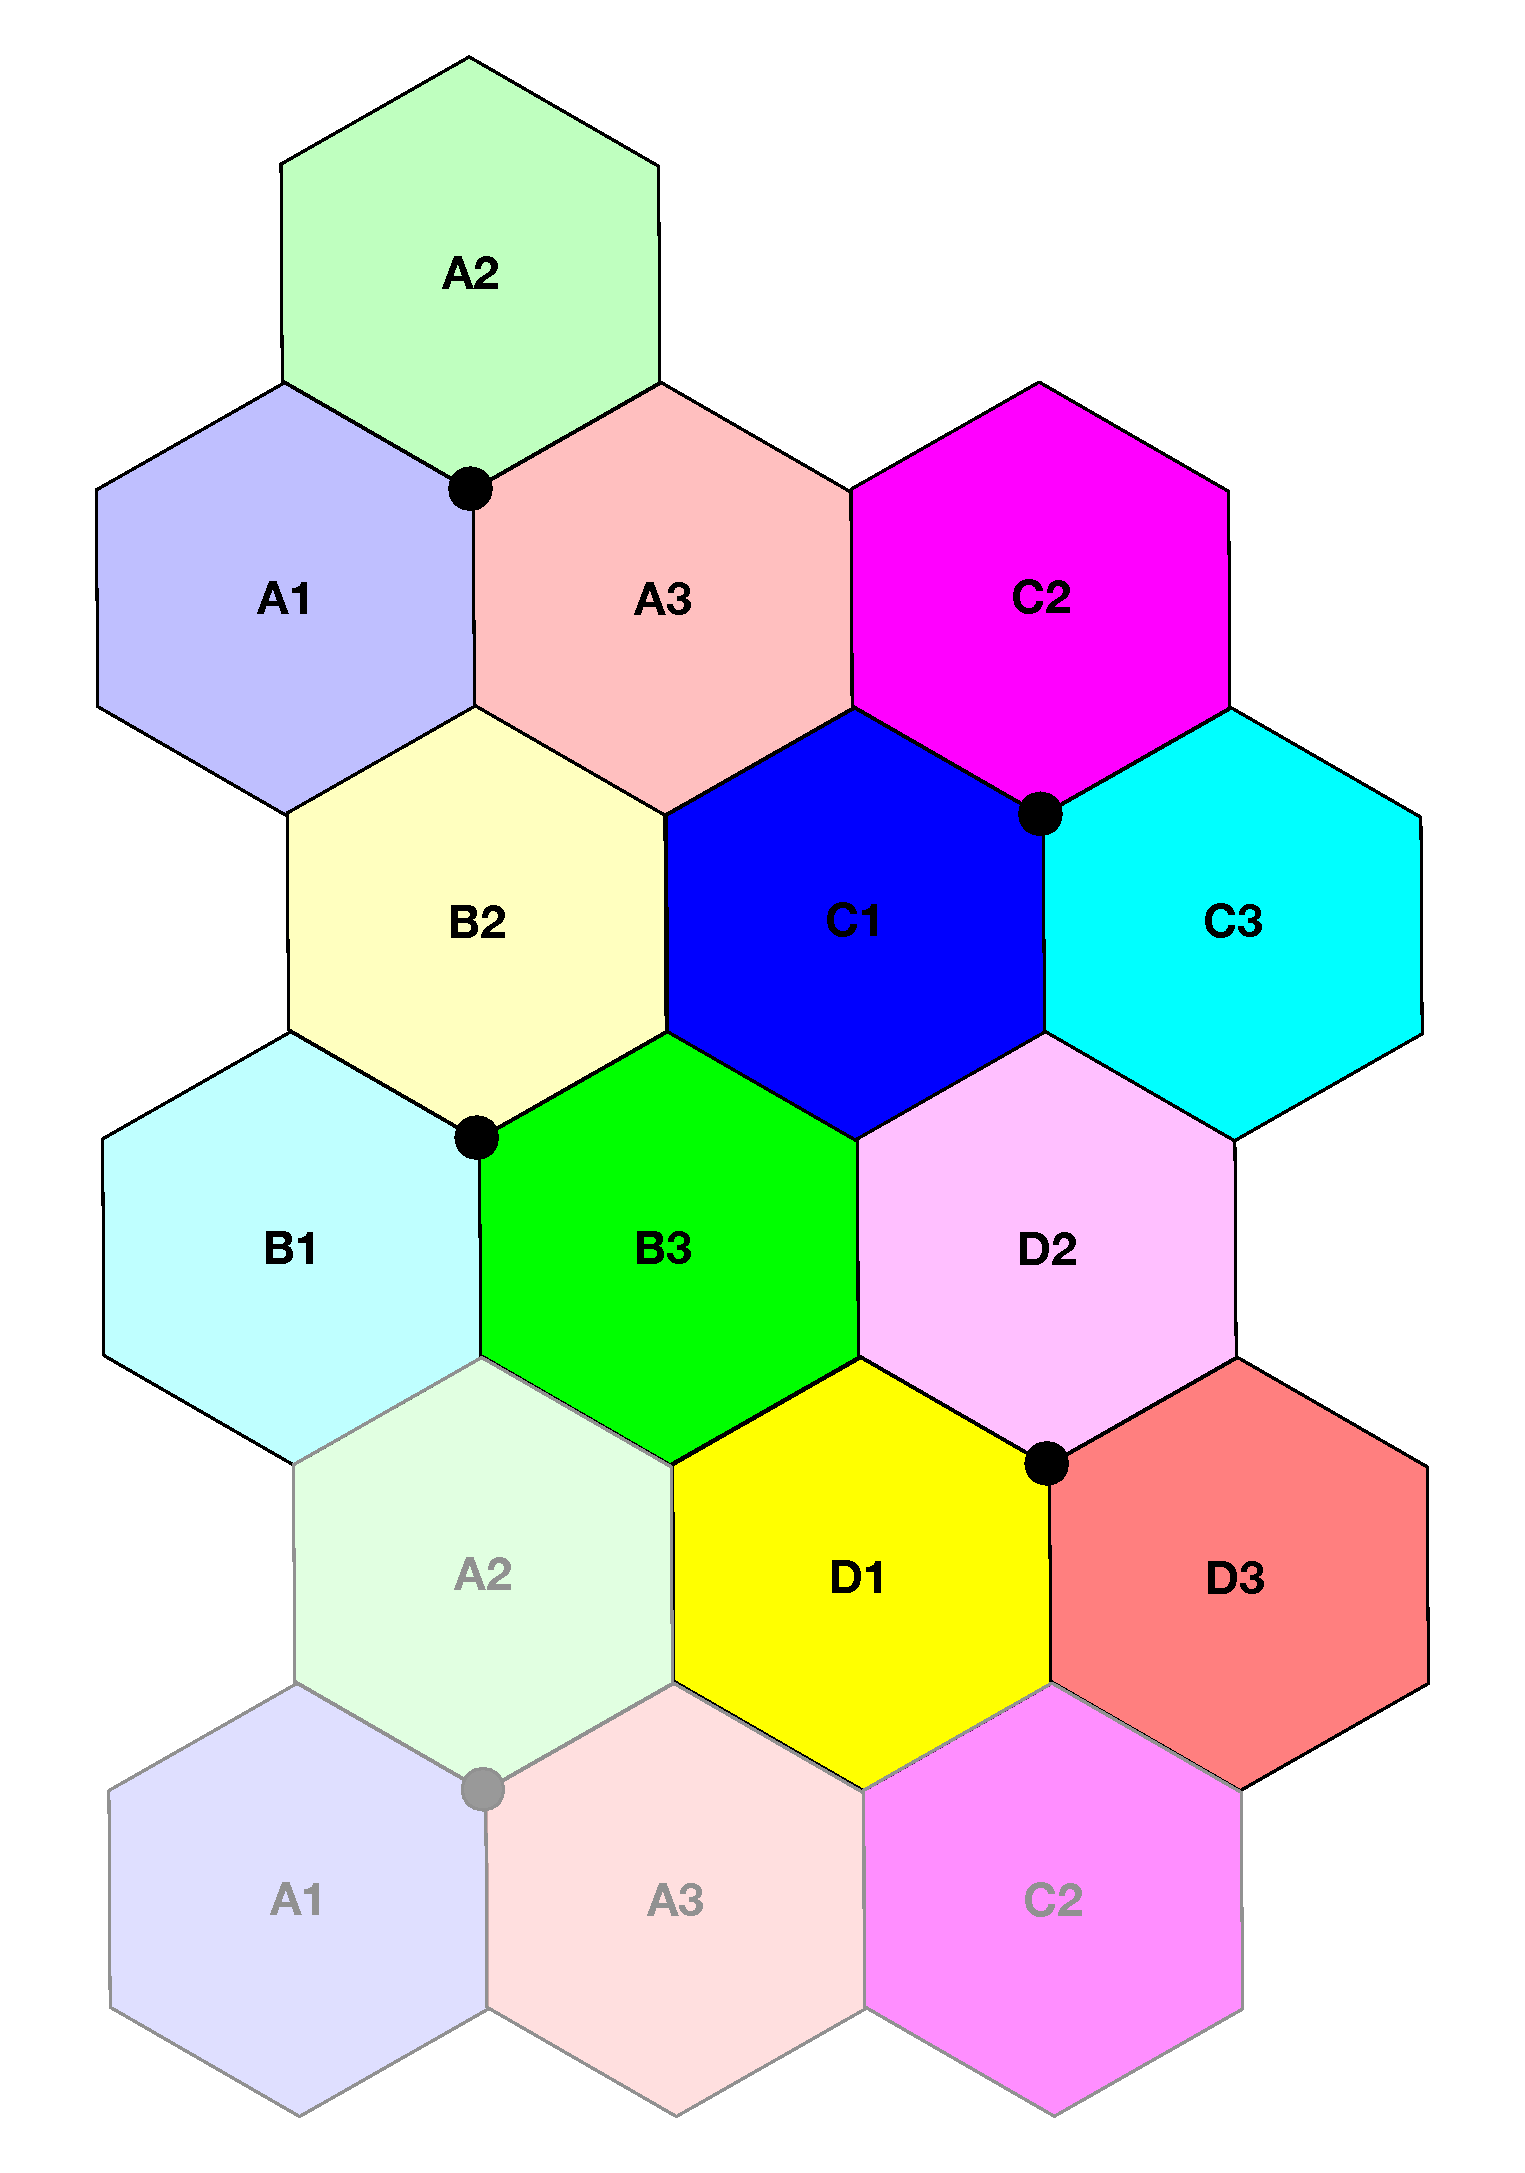
\includegraphics[width=0.4\linewidth]{../Apuntes/Figuras/SDMA.pdf}
\end{frame}


\section{CDMA}
\subsection{Introducción}
\begin{frame}{CDMA (Code Division Multiple Access)}{Introducción}
  \begin{itemize}
    \item Los usuarios transmiten simultáneamente y en las mismas frecuencias.
    \item ¿Cómo se separa cada comunicación?
    \begin{itemize}
      \item Técnicas de espectro ensanchado (SS, Spread Spectrum):
      \begin{itemize}
        \item {\bf DS}: Direct Sequence
        \item {\bf FH}: Frequency Hoping
        \item {\bf TH}: Time Hoping
      \end{itemize}
    \end{itemize}
  \end{itemize}
\end{frame}

\subsection{Técnicas DS}
\begin{frame}{CDMA}{Técnicas DS}
  \begin{itemize}
    \item Cada usuario dispone de un código que utiliza para codificar la señal enviada:
  \end{itemize}
  \centering 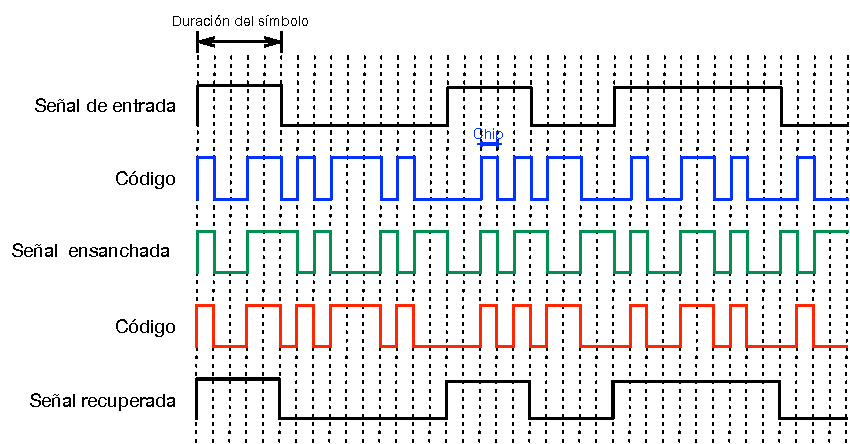
\includegraphics[width=0.8\linewidth]{../Apuntes/Figuras/DS-CDMA.pdf}
\end{frame}

\begin{frame}{CDMA}{Técnicas DS}
  \begin{itemize}
    \item Sólo aquellos usuarios con el código correcto podrán interpretar la señal recibida.
    \item Para el resto será indistinguible del ruido.
    \item La probabilidad de error para M usuario es:\\
    \begin{displaymath}
      P_e = Q \left ( \frac{1}{\sqrt{\frac{M-1}{3P_g} + \frac{N_0}{2E_b}}} \right )
    \end{displaymath}
    (siendo $P_g = \frac{W_c}{W_x}$ la ganancia del proceso)

    \item Si no hay ruido, la probabilidad de error se simplifica:
    \begin{displaymath}
      P_e = Q \left ( \sqrt{\frac{3P_g}{M-1}} \right )
    \end{displaymath}
  \end{itemize}
\end{frame}

\subsection{Problema cerca-lejos}
\begin{frame}{CDMA}{Problema cerca-lejos}
  \begin{itemize}
    \item Es uno de los principales problemas de los sistemas CDMA
    \item Caso típico: telefonía móvil
    \item Puede haber problemas al detectar una señal débil en presencia de otras de mayor potencia
    \item Solución: técnicas de control de potencia
    \item Ventaja añadida: ahorro de batería
  \end{itemize}
\end{frame}

\subsection{Técnicas FH}
\begin{frame}{CDMA}{Tecnicas FH (Frequency Hoping)}
  \begin{itemize}
    \item Surgieron en la II Guerra Mundial como técnicas para guiar torpedos sin poder ser detectados por el enemigo.
    \item La señal va saltando de una frecuencia a otra siguiendo una secuencia pseudoaleatoria
  \end{itemize}
  \centering 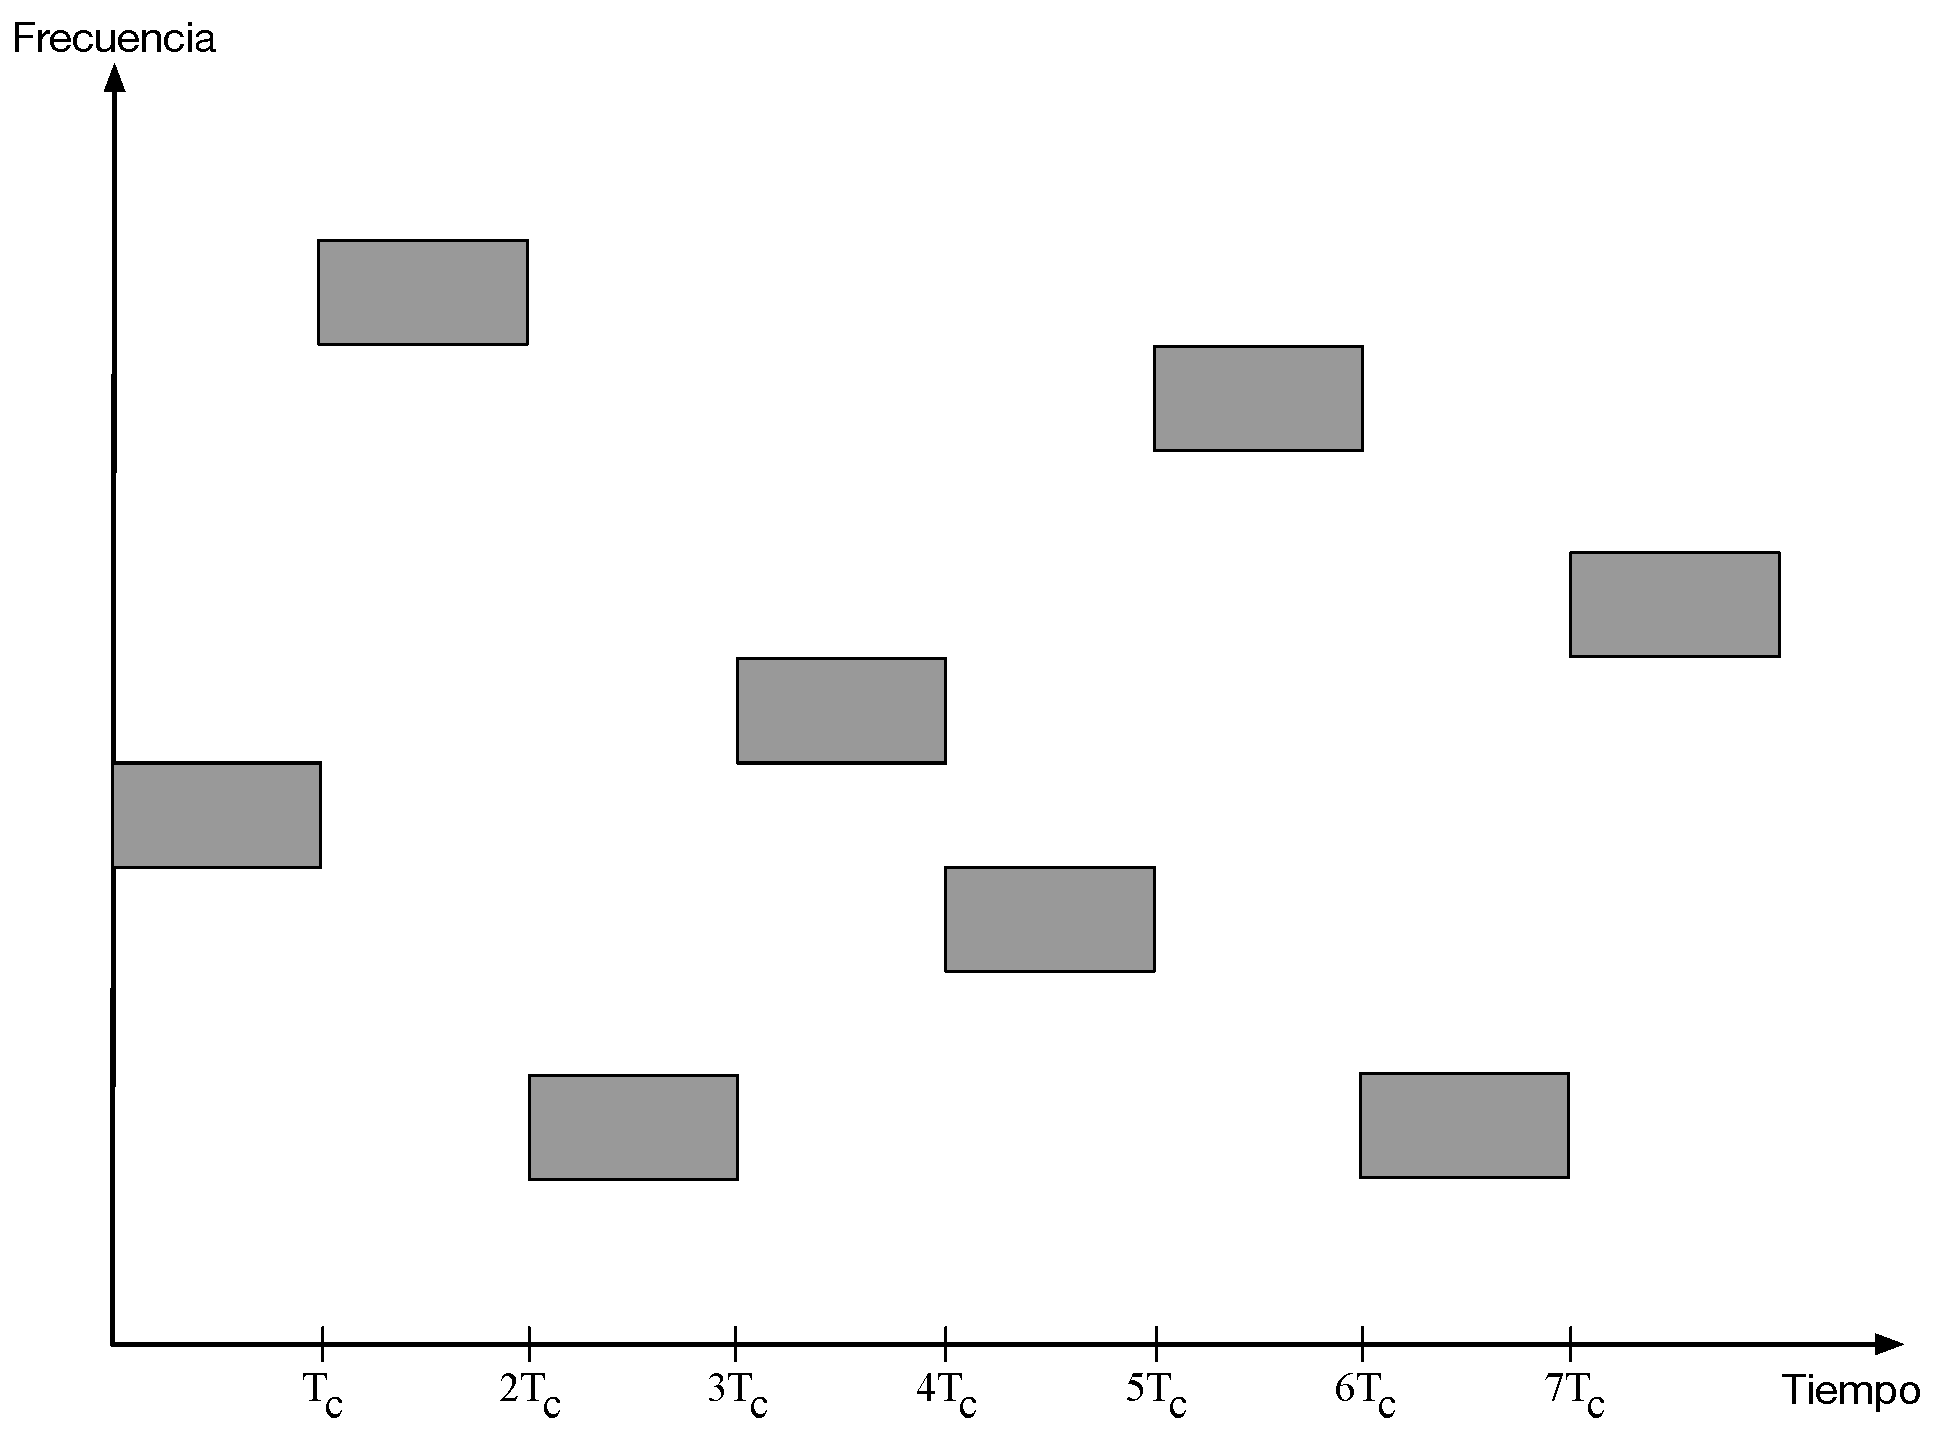
\includegraphics[width=0.5\linewidth]{../Apuntes/Figuras/FrequencyHoping.pdf}
\end{frame}

\subsection{Ventajas e inconvenientes}
\begin{frame}{CDMA}{Ventajas e inconvenientes}
  \begin{itemize}
    \item Ventajas:
      \begin{itemize}
        \item Señal transmitida con baja densidad espectral de potencia $\Rightarrow$ afecta poco a otros sistemas.
        \item Privacidad
        \item No existen slots de transmisión
        \item Uso eficiente del espectro
        \item Disminución de problemas por multitrayecto $\Rightarrow$ Receptor RAKE
      \end{itemize}
    \item Inconvenientes:
      \begin{itemize}
        \item El rendimiento se degrada al aumentar los usuarios
        \item Problema cerca-lejos
      \end{itemize}
  \end{itemize}
\end{frame}

\section{OFDMA}
\subsection{Introducción}
\begin{frame}{OFDMA (Orthogonal Frequency Division Multiple Access)}{Introducción}
  \begin{itemize}
    \item Los datos se reparten entre varias subportadoras ortogonales y equiespaciadas en frecuencia:
    \begin{displaymath}
      \int_0^T cos \left ( 2\pi f_k t\right ) cos \left ( 2\pi f_i t\right ) = 0 \, \, \forall k \neq i
    \end{displaymath}
    \item Cada subportadora funciona como un canal que transporta sus propios datos
    \item Puede verse como una técnica de espectro ensanchado
  \end{itemize}
\end{frame}

\subsection{Funcionamiento}
\begin{frame}{OFDMA}{Funcionamiento}
  \begin{itemize}
    \item ¿Cómo se aplica esta idea al acceso mútiple?
    \item Se asigna a cada usuario un cierto número de portadoras entre las que reparte el flujo total de datos
    \item Cada subflujo modula a cada portadora
    \item A cada usuario se le puede asignar, en cada slot de tiempo, un cierto número de portadoras ortogonales
  \end{itemize}
\end{frame}

\subsection{Funcionamiento}
\begin{frame}{OFDMA}{Funcionamiento}
  \begin{itemize}
    \item Espectro de 8 señales OFDM:
  \end{itemize}
  \centering 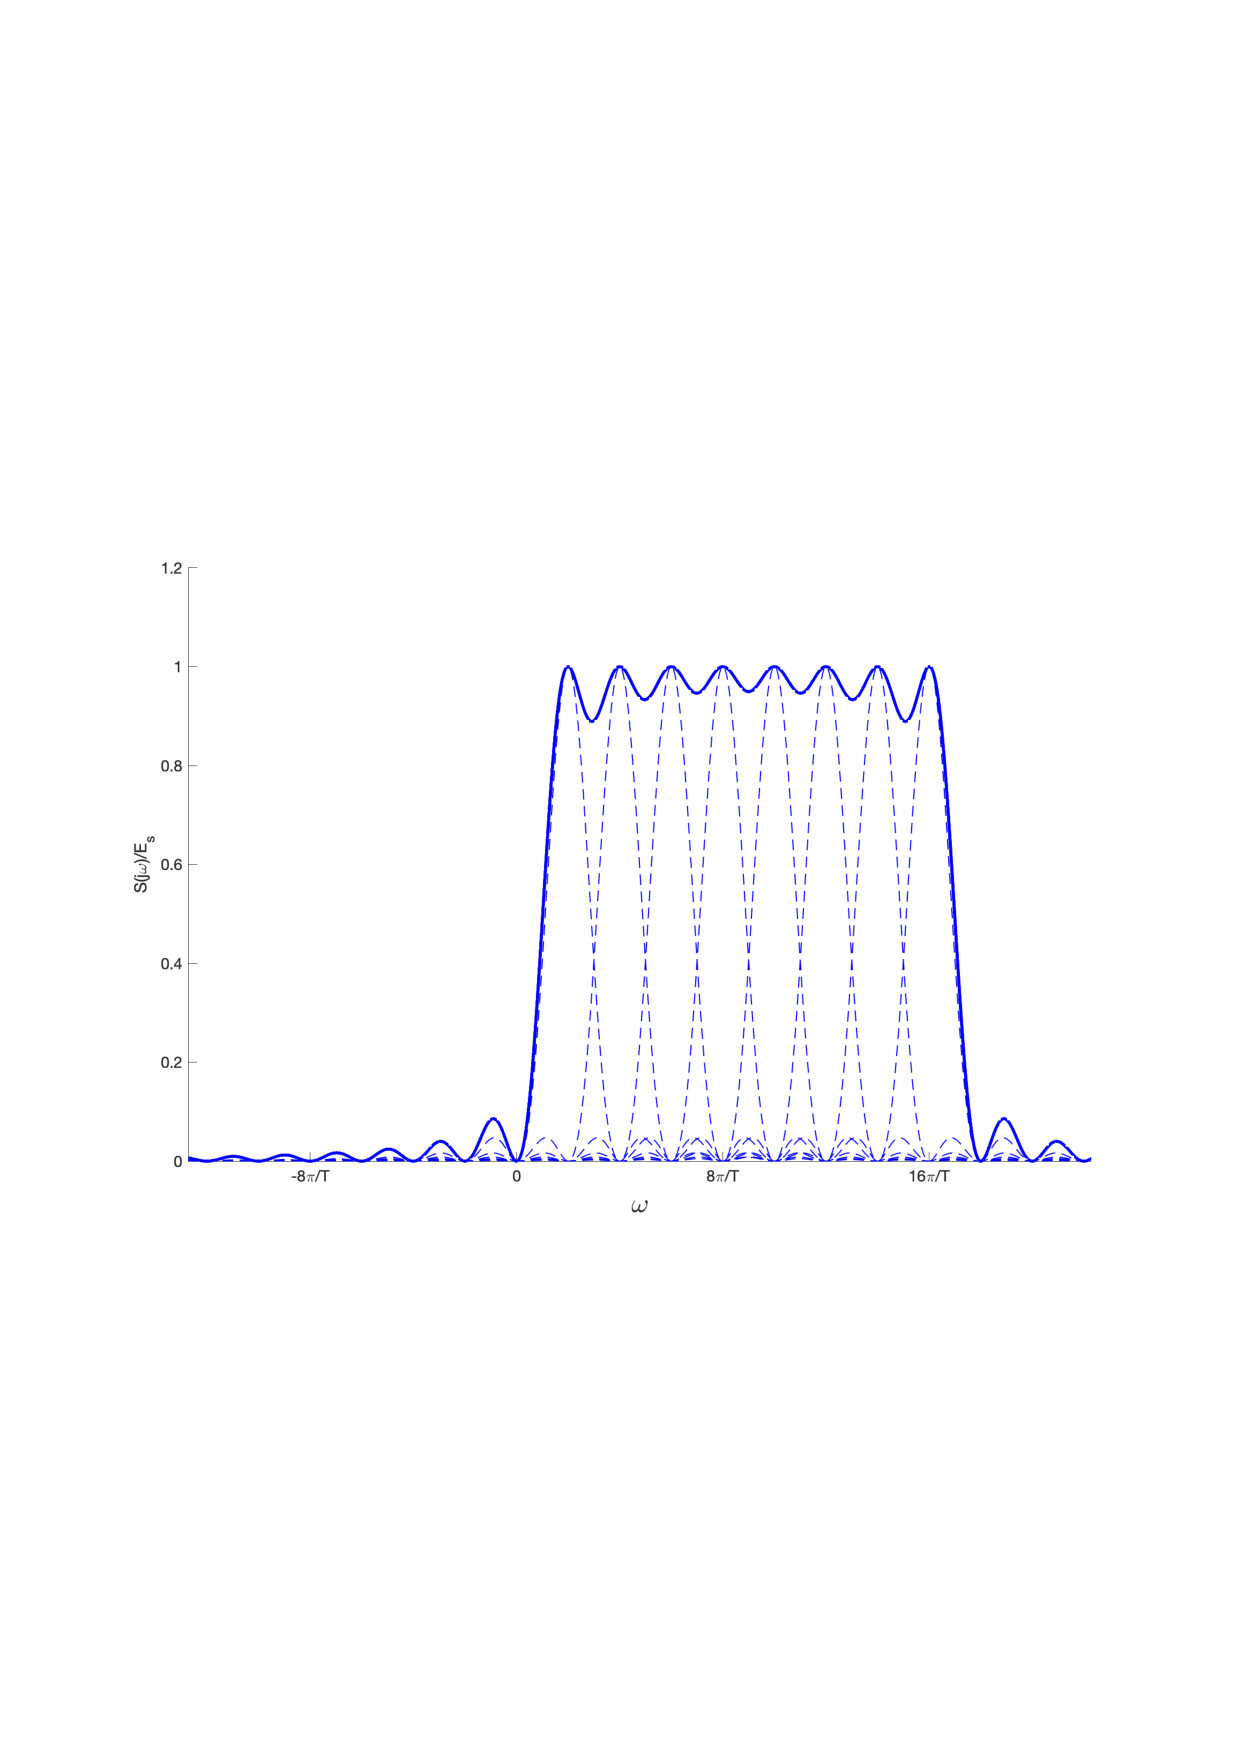
\includegraphics[width=0.8\linewidth]{../Apuntes/Figuras/OFDM.pdf}
\end{frame}

\subsection{Número de usuarios}
\begin{frame}{OFDMA}{Número de usuarios}
  \begin{itemize}
    \item Según en teorema de Nyquist generalizado, el número máximo de usuarios es $2WT$ (siendo $W$ el ancho de banda)
    \item ¿Cómo se puede ampliar este número?
      \begin{itemize}
        \item No asignar las portadoras de forma permanente
        \begin{itemize}
          \item Técnicas CSMA/CD (Carrier Sense Multiple Access with Collision Detection). Ej. Ethernet
        \end{itemize}
        \item Usar señales ``casi'' ortogonales $\Rightarrow$ Interferencia multiacceso (MAI).
      \end{itemize}
  \end{itemize}
\end{frame}


\subsection{Ventajas e inconvenientes}
\begin{frame}{OFDMA}{Ventajas e inconvenientes}
  \begin{itemize}
    \item Ventajas:
      \begin{itemize}
        \item Se reduce el riesgo de interferencia entre subcanales
        \item Robusto frente a multitrayecto
        \item No es necesario utilizar filtros pasobanda como en FDMA
      \end{itemize}
    \item Inconvenientes:
      \begin{itemize}
        \item Es necesaria una sincronización estricta
      \end{itemize}
    \item Aplicaciones:
      \begin{itemize}
        \item Wi-Fi (IEEE 802.11)
        \item WiMax (IEEE 802.16)
      \end{itemize}
  \end{itemize}
\end{frame}

\subsection{OFDMA vs. FDMA}
\begin{frame}{OFDMA}{OFDMA vs. FDMA}
  \begin{itemize}
    \item OFDMA es {\bf más eficiente} en ancho de banda
    \item OFDMA permite {\bf mayor velocidad} de datos 
    \item OFDMA es {\bf menos robusto} frente a interferencia multitrayecto
  \end{itemize}
\end{frame}

\subsection{OFDMA vs. CDMA}
\begin{frame}{OFDMA}{OFDMA vs. CDMA}
  \begin{itemize}
    \item En OFDMA la información se transmite utilizando varias {\bf portadoras ortogonales}
    \item En CDMA todos los usuarios {\bf comparten frecuencias} y se utilizan códigos
    \item CDMA permite {\bf comunicaciones más seguras} en entornos ruidosos
  \end{itemize}
\end{frame}


\section{NOMA}
\subsection{Introducción}
\begin{frame}{NOMA (Non-Orthogonal Multiple Access)}{Introducción}
  \centering 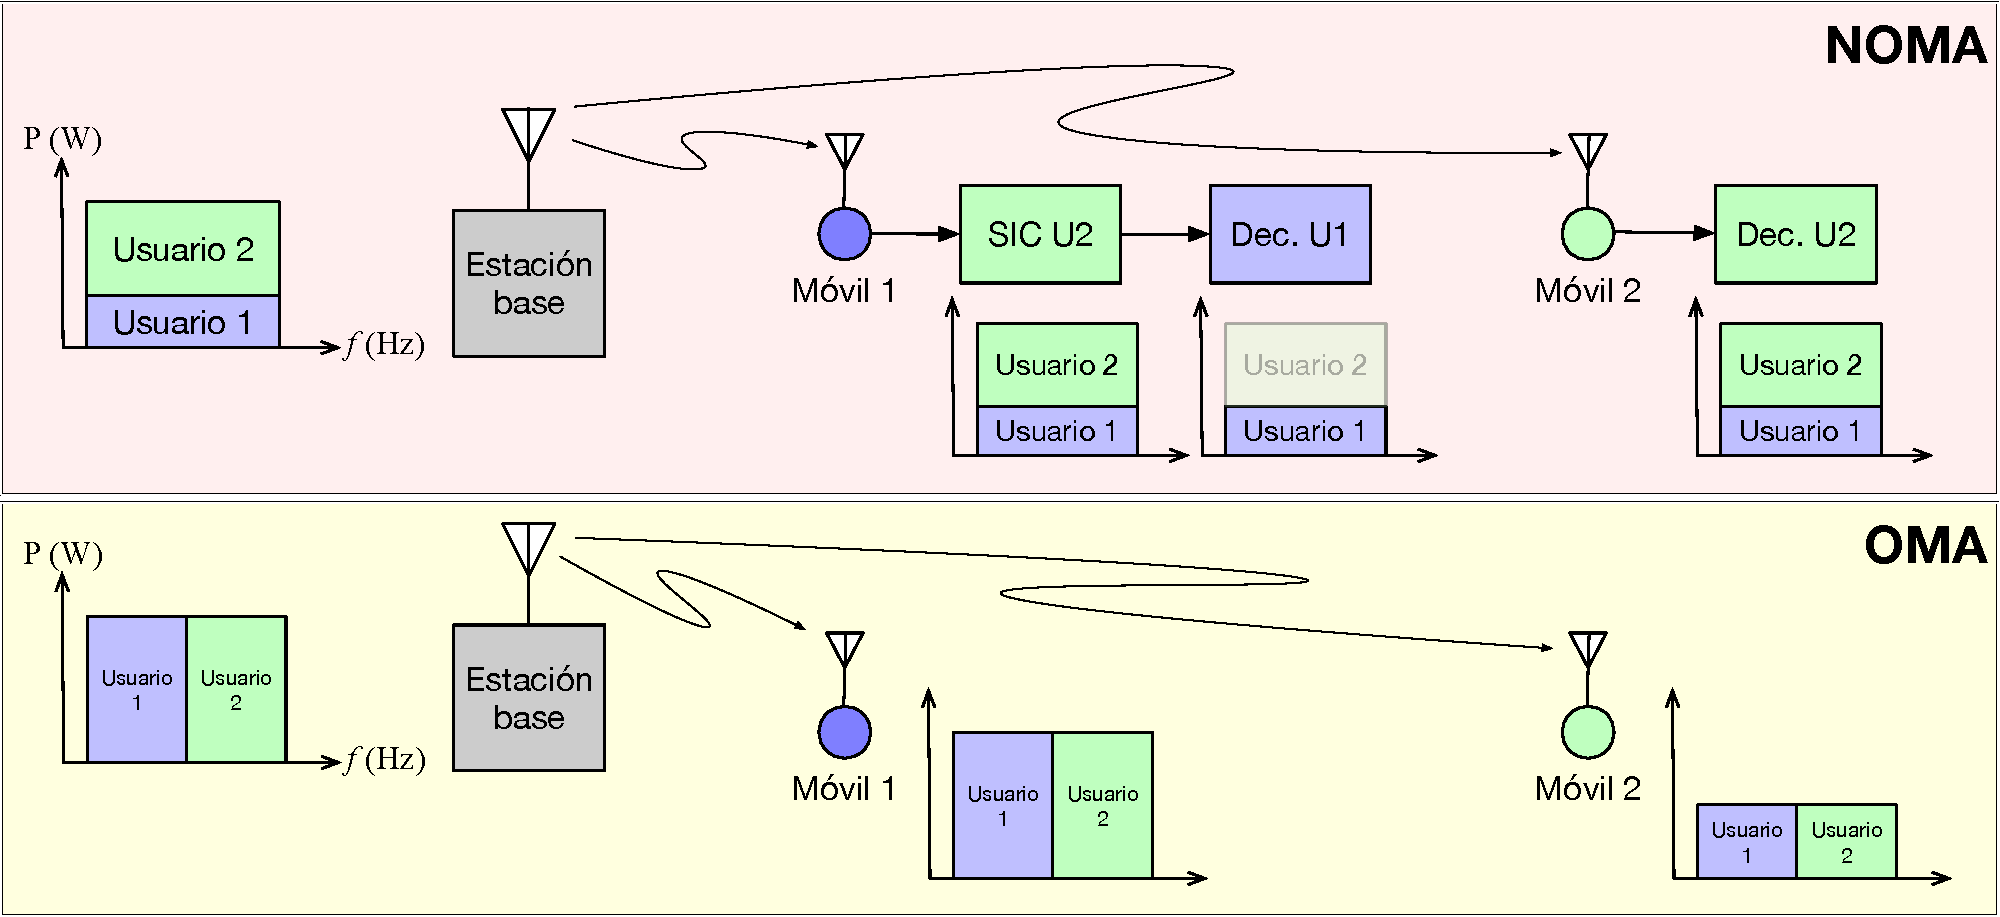
\includegraphics[width=0.8\linewidth]{../Apuntes/Figuras/NOMA.pdf}
\end{frame}

\subsection{NOMA vs. OMA}
\begin{frame}{NOMA}{NOMA vs. OMA}
  \begin{itemize}
    \item En OMA, cada frecuencia se asigna a un usuario, aunque tenga malas condiciones de canal $\Rightarrow$ {\bf Afecta a todo el sistema}
    \begin{itemize}
      \item NOMA comparte la misma frecuencia con todos los usuarios
    \end{itemize}
    \item En OMA, los usuarios con mejores condiciones de canal tienen mayor prioridad $\Rightarrow$ {\bf Problema con conexiones masivas}
    \begin{itemize}
      \item NOMA proporciona mejores condiciones y menor latencia
    \end{itemize}
    \item NOMA es {\bf prácticamente compatible} con las arquitecturas actuales
  \end{itemize}
\end{frame}


\subsection{NOMA vs. OFDMA}
\begin{frame}{NOMA}{NOMA vs. OFDMA}
  \centering 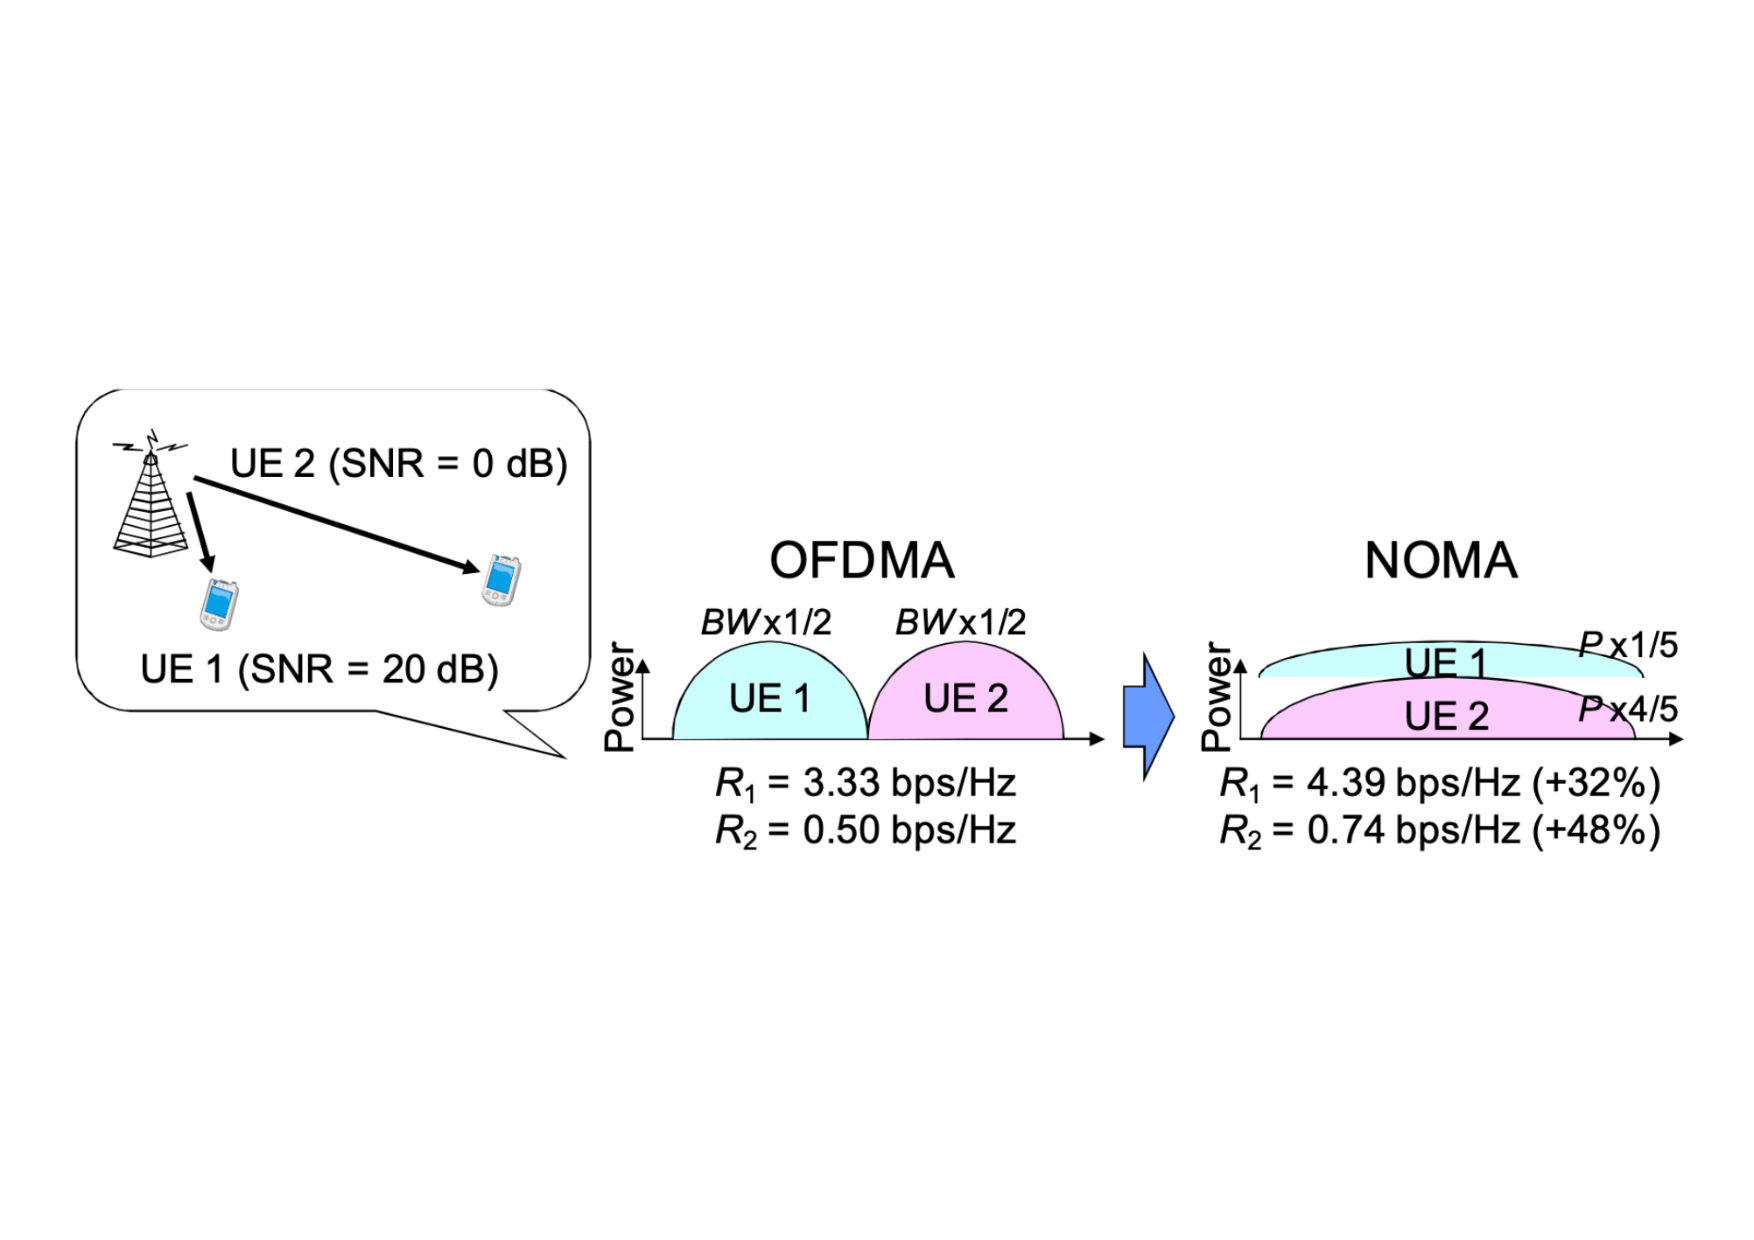
\includegraphics[width=0.8\linewidth]{../Apuntes/Figuras/NOMA_OFDMA.pdf}
\end{frame}
\end{document}
